\subsection{Product of a space by a simply connected space}

PROPOSITION 8. --- Let B be a topological space. Let T be a simply connected and locally connected space. Let E be a covering of B × T, with projection p, and let t be a point of T. Denote by \(E_{t}\) the space \(p^{-1}(B \times \{t\})\) equipped with the map \(p_{t} = pr_{1} \circ p \mid E_{t}: E_{t} \to B\) ; this is a covering of B. There then exists a unique (B × T)-isomorphism from the covering ( \(E_{t} \times T, p_{t} \times Id_{T}\) ) onto the covering E which maps (x, t) to x for all \(x \in E_{t}\) .

One may assume that B is nonempty. Let \(x\) be a point of \(E_t\) . By Proposition 3 of I, p. 125 applied to the covering E and the continuous map T → B × T, \(u \mapsto (p_t(x), u)\) , there exists a unique continuous map \(f_x \colon \mathrm{T} \to \mathrm{E}\) such that \(f_x(t) = x\) and \(p(f_x(u)) = (p_t(x), u)\) for all \(u \in T\) . Let \(h \colon E_t \times T \to E\) be the map defined by \(h(x, u) = f_x(u)\) . We have \(h(x, t) = x\) and \(p \circ h = p_t \times \operatorname{Id}_T\) . The map h is a lift to E of the map \(p_t \times \operatorname{Id}_T\) . The restriction of h to \(E_t \times \{t\}\) is continuous, as is the restriction of h to \(\{x\} \times T\) for every point x of \(E_t\) . Since the space T is locally connected, the map h is continuous (I, p. 37, cor. 1 of th. 1).

Let \(b\) be a point of B. By construction, the map \(h\) induces a bijection from the fiber \(p_t^{-1}(b) \times \{t\}\) of \(E_t \times T\) onto the fiber \(p^{-1}(b,t)\) of E at \((b,t)\) . Since the space T is connected and locally connected, the map \(h\) is bijective (I, p. 84, cor. of prop. 7). It is therefore a \(B \times T\) -isomorphism (I, p. 30, cor. 2 of prop. 6).

Let \(h'\) be a \((\mathrm{B} \times \mathrm{T})\) -isomorphism from the covering \((\mathrm{E}_{t} \times \mathrm{T}, p_{t} \times \mathrm{Id}_{\mathrm{T}})\) onto the covering E which maps \((x, t)\) to x for every point \(x \in E_{t}\) . For all \(x \in E_{t}\) , the maps \(u \mapsto h(x, u)\) and \(u \mapsto h'(x, u)\) are equal (I, p. 34, cor. 1 of prop. 11). We therefore have \(h = h'\) .

COROLLARY 1. --- Under the hypotheses of Prop. 8, if t and t' are two points of T, the coverings \(E_{t}\) and \(E_{t'}\) are B-isomorphic.

COROLLARY 2. --- Under the hypotheses of Prop. 8, let (E,p) and (E',p') be coverings of B × T and let \(k: E_t \to E_t'\) be a B-morphism. There exists a unique (B × T)-morphism \(\widetilde{k}\) : E → E' which extends k. If k is a B-isomorphism, \(\widetilde{k}\) is a (B × T)-isomorphism.

By proposition 8, we may assume that there exist coverings F and F′ of B such that E and E′ are respectively the (B × T)-spaces F × T and F′ × T. We then have \(E_{t} = F \times \{t\}\) , \(E_{t}' = F' \times \{t\}\) and the map k is written \((x, t) \mapsto (k'(x), t)\) , where \(k'\) is a B-morphism from F into F'. The map \(k' \times Id_{T}\) is a B × T-morphism extending k; it is an isomorphism if k is one.

Let \(\widetilde{k}\colon\mathrm{E}\to\mathrm{E}^{\prime}\) be a \((\mathrm{B}\times\mathrm{T})\) -morphism extending \(k\) . Let \(x\) be a point of F. Denote by \(q\) the projection of F and set \(b=q(x)\) . The maps \(u\mapsto\widetilde{k}(x,u)\) and \(u\mapsto(k^{\prime}(x),u)\) are liftings in \(\mathrm{E}^{\prime}\) of the map \(u\mapsto(b,u)\) from T to \(\mathrm{B}\times\mathrm{T}\) . They coincide at \(t\) . Since the space T is connected, they are equal. Thus, \(\widetilde{k}\) is the \((\mathrm{B}\times\mathrm{T})\) -morphism \(k^{\prime}\times\mathrm{Id}_{\mathrm{T}}\colon\mathrm{F}\times\mathrm{T}\to\mathrm{F}^{\prime}\times\mathrm{T}\) .

COROLLARY 3. --- Let B and B' be topological spaces, let T be a simply connected and locally connected topological space. Let \(f: B' \times T \to B\) be a continuous map and let E be a covering of B. Given a point t of T and a continuous lifting \(g_t: B' \times \{t\} \to E\) of \(f | B' \times \{t\}\) to E, there exists a unique continuous lifting g of f to E extending \(g_t\) .

In view of prop. 3 of I, p. 9, it suffices to show that every continuous section of \(f^{*}(\mathrm{E})\) over \(\mathrm{B}' \times \{t\}\) extends uniquely to a continuous section of \(f^{*}(\mathrm{E})\) . Now this follows from cor. 2 applied to the coverings \((\mathrm{B}' \times \mathrm{T}, \mathrm{Id}_{\mathrm{B}' \times \mathrm{T}})\) and \(f^{*}\mathrm{E}\) of \(\mathrm{B}' \times \mathrm{T}\) .

Remark. --- Keep the hypotheses and notation of Proposition 8. Let G be a discrete topological group. Suppose that E is a principal covering with group G. If one equips the coverings \(E_{t}\) of B and \(E_{t} \times T\) of \(B \times T\) with principal covering structures of group G deduced from that of E (I, p. 92, examples 1 and 4), then the coverings E and \(E_{t} \times T\) are isomorphic principal coverings. Indeed, let \(h: E_{t} \times T \to E\) be the unique (B × T)-morphism such that \(h(x, t) = x\) for all \(x \in E_{t}\) . For every element g of G, the map \((x, u) \mapsto h(x \cdot g, u) \cdot g^{-1}\) is a (B × T)-morphism that maps \((x, t)\) to x for all \(x \in E_{t}\) and therefore is equal to h. This proves that h is a (B × T)-morphism of principal coverings.

In particular, under the preceding hypotheses, the principal coverings \(E_{t}\) and \(E_{t'}\) are isomorphic, for \(t' \in T\) . Similarly, one proves that if, in Corollary 2, E and \(E'\) are principal coverings with group G and if k is a B-isomorphism of principal coverings with group G, \(\widetilde{k}\) is a \((\mathrm{B} \times \mathrm{T})\) isomorphism of principal coverings.

PROPOSITION 9. --- Let B be a topological space and let (E,p) be a covering of B. Let T be a simply connected, locally connected, and locally compact topological space. Denote by \(\widetilde{p}\colon\mathcal{C}_{c}(\mathrm{T};\mathrm{E})\to\mathcal{C}_{c}(\mathrm{T};\mathrm{B})\) the map \(g\mapsto p\circ g\) . Let t be a point of T. Denote \(e_{\mathrm{E}}\colon\mathcal{C}_{c}(\mathrm{T};\mathrm{E})\to\mathrm{E}\) the map which to \(g\in\mathcal{C}_{c}(\mathrm{T};\mathrm{E})\) associates \(g(t)\) , and \(e_{\mathrm{B}}\colon\mathcal{C}_{c}(\mathrm{T};\mathrm{B})\to\mathrm{B}\) the map which to \(f\in\mathcal{C}_{c}(\mathrm{T};\mathrm{B})\) associates \(f(t)\) .

The square

\[
\begin{array}{c} \mathcal {C} _ {c} (\mathrm{T}; \mathrm{E}) \xrightarrow {e _ {\mathrm{E}}} \mathrm{E} \\ \Big \downarrow \widetilde {p} \\ \mathcal {C} _ {c} (\mathrm{T}; \mathrm{B}) \xrightarrow {e _ {\mathrm{B}}} \mathrm{B} \end{array}
\]

is Cartesian.

Let us first prove a lemma.

Lemma. --- Let X, Y, Z be topological spaces and let \(g: Y \rightarrow Z\) be a continuous map.

\begin{enumerate}
\def\labelenumi{\alph{enumi})}
\item
  The map \(f\mapsto g\circ f\) from \(\mathcal{C}_c(\mathrm{X};\mathrm{Y})\) to \(\mathcal{C}_c(\mathrm{X};\mathrm{Z})\) is continuous.
\item
  If the topological space Z is Hausdorff, the map \(h \mapsto h \circ g\) from \(\mathcal{C}_{c}(\mathrm{Z};\mathrm{X})\) to \(\mathcal{C}_{c}(\mathrm{Y};\mathrm{X})\) is continuous.
\end{enumerate}

Given a compact subset K of X, an open subset U of Z, and a continuous map f from X to Y, in order to have \((g \circ f)(\mathrm{K}) \subset \mathrm{U}\) , it is necessary and sufficient that one have \(f(\mathrm{K}) \subset g^{-1}(\mathrm{U})\) . The first assertion therefore follows from the definition of the topology of compact convergence (TG, X, p. 26, def. 1).

Similarly, let K be a compact subset of Y and U an open subset of X. Since the space Z is assumed to be Hausdorff, the set \(g(\mathrm{K})\) is compact (TG, I, p. 63, cor. 1). If h is a mapping from Z into X, the condition \((h \circ g)(\mathrm{K}) \subset \mathrm{U}\) is none other than the condition \(h(g(\mathrm{K})) \subset \mathrm{U}\) , whence the second assertion.

Let us now prove Proposition 9. By the lemma, the map \(\widetilde{p}\) is continuous; by Remark 1 of TG, X, p. 27, the maps \(e_{\mathrm{E}}\) and \(e_{\mathrm{B}}\) are continuous. For any map \(g \in \mathcal{C}_c(\mathrm{T};\mathrm{E})\) , we have

\[
(p \circ e _ {\mathrm{E}}) (g) = p (g (t)) = (p \circ g) (t) = \widetilde {p} (g) (t) = \left(e _ {\mathrm{B}} \circ \widetilde {p}\right) (g),
\]

so that the square diagram of the proposition is commutative.

Let \(\varphi\colon\mathcal{C}_{c}(\mathrm{T};\mathrm{E})\to\mathcal{C}_{c}(\mathrm{T};\mathrm{B})\times_{\mathrm{B}}\mathrm{E}\) be the continuous map defined by \(\varphi(g)=(p\circ g,g(t))\) for all \(g\in\mathcal{C}_{c}(\mathrm{T};\mathrm{E})\) . By Proposition 3 of I, p. 125, it is bijective. Indeed, for every pair \((f,x)\in\mathcal{C}_{c}(\mathrm{T};\mathrm{B})\times_{\mathrm{B}}\mathrm{E},\varphi^{-1}(f,x)\) is the unique continuous lift \(g\) of \(f\) to E such that \(g(t)=x\) . Since the space T is locally compact, the map \(\psi\colon(\mathcal{C}_{c}(\mathrm{T};\mathrm{B})\times_{\mathrm{B}}\mathrm{E})\times\mathrm{T}\to\mathrm{B}\) defined by \(\psi((f,x),u)=f(u)\) is continuous (TG, X, p. 28, cor. 1). By Corollary 3 above, the map \(\psi\) has a unique continuous lift \(\theta\colon(\mathcal{C}_{c}(\mathrm{T};\mathrm{B})\times_{\mathrm{B}}\mathrm{E})\times\mathrm{T}\to\mathrm{E}\) such that \(\theta((f,x),t)=x\) for \((f,x)\in\mathcal{C}_{c}(\mathrm{T};\mathrm{B})\times_{\mathrm{B}}\mathrm{E}\) . One thus has \(\theta((f,x),u)=\varphi^{-1}(f,x)(u)\) for \((f,x)\in\mathcal{C}_{c}(\mathrm{T};\mathrm{B})\times_{\mathrm{B}}\mathrm{E}\) and \(u\in\mathrm{T}\) . By Theorem 3 of TG, X, p. 28, the map \((f,x)\mapsto\theta((f,x),\cdot)\) from \(\mathcal{C}_{c}(\mathrm{T};\mathrm{B})\times_{\mathrm{B}}\mathrm{E}\) to \(\mathcal{C}_{c}(\mathrm{T};\mathrm{E})\) is continuous, that is, \(\varphi^{-1}\) is continuous.

Thus, the map \(\varphi\) is a homeomorphism from \(\mathcal{C}_c(\mathrm{T};\mathrm{E})\) onto the fibered product \(\mathcal{C}_c(\mathrm{T};\mathrm{B})\times_{\mathrm{B}}\mathrm{E}\) , whence the proposition (I, p. 8, prop. 2).

\subsection{Homeomorphism groups of simply connected spaces}

Let X be a connected nonempty topological space, and let G be a discrete group acting continuously on the left on X; denote by e the identity element of G. Let M be a subset of X such that \(G \cdot M = X\) . We set

\[
\mathrm{S} = \{g \in \mathrm{G} \mid g \cdot \mathrm{M} \cap \mathrm{M} \neq \varnothing \}.
\]

We have \(e \in S\) and \(S = S^{-1}\) .

For every \(x \in X\) , denote by \(E_{x}\) the set of \(g \in G\) such that \(x \in g \cdot M\) . Let \(g, h \in E_{x}\) ; then \(g \cdot M \cap h \cdot M \neq \varnothing\) , so that \(g^{-1}h \in S\) . In particular, for every \(x \in M\) , we have \(e \in E_{x}\) whence \(E_{x} \subset S\) .

We make one of the following two hypotheses:

\begin{enumerate}
\def\labelenumi{(\roman{enumi})}
\item
  The set M is open;
\item
  The set M is closed and the covering \((g \cdot \mathrm{M})_{g \in \mathrm{G}}\) of X is locally finite.
\end{enumerate}

Lemma 2. --- For every point \(x \in X\) , the map \(\mu_x: E_x \times M \to X\) given by \((g, u) \mapsto g \cdot u\) is universally strict, and its image \(E_x \cdot M\) is a neighbourhood of \(x\) in \(X\) . In particular, \(S \cdot M\) is a neighbourhood of \(M\) .

Under assumption (i), the map \(\mu_{x}\) is open, since \(E_{x} \times M\) is open in \(G \times M\) . Its image is then open in X.

Suppose now that hypothesis (ii) is satisfied. The map \(\mu_x\) is proper (TG, I, p. 6, prop. 4, and p. 75, th. 1), hence universally strict (I, p. 20, corollary 11). Moreover, \((\mathrm{G} - \mathrm{E}_x) \cdot \mathrm{M}\) is a closed subset of X that does not contain \(x\) , so that \(\mathrm{E}_x \cdot \mathrm{M}\) is a neighbourhood of \(x\) .

The last assertion follows from the fact that \(E_{x} \subset S\) if \(x \in M\) .

Lemma 3. --- The group G is generated by S.

Let H be the subgroup of G generated by S. Let U = H·M ; observe that U is the union of the subsets of the form \(h \cdot (S \cdot M)\) , for \(h \in H\) . Since S · M is a neighbourhood of M (lemma 2), the set U is a neighbourhood of H · M = U ; it follows that U is open in X. Let \(g, g' \in G\) such that \(g \cdot U \cap g' \cdot U \neq \varnothing\) ; let \(h, h' \in H\) and \(x, x' \in M\) such that \(gh \cdot x = g'h' \cdot x'\) ; then \(h^{-1}g^{-1}g'h' \cdot x' = x\) , so that \(h^{-1}g^{-1}g'h' \in S\) ; in particular, \(g^{-1}g' \in H\) . When \(g\) runs through a system of representatives of the left cosets modulo \(H\) , the sets \(g \cdot U\) are thus pairwise disjoint; since \(G \cdot M = X\) , they cover \(X\) . Since \(X\) is connected, it follows that \((G : H) = 1\) , whence \(H = G\) .

Let T be the set of pairs \((s,t)\) of elements of G such that \(M\cap s\cdot M\cap st\cdot M\neq\varnothing\) ; if \((s,t)\in\mathrm{T}\) , then s, t, and st belong to S. Let F be the group \(\mathrm{F}(\mathrm{S},\mathbf{r})\) defined by the generating set S and by the set r of relations \(str^{-1}\) for \(r,s,t\in S\) such that \((s,t)\in\mathrm{T}\) and r=st; denote \(\varepsilon\) its identity element and \(\varphi\colon F\to G\) the canonical homomorphism (A, I, p. 86, prop. 9). If \(s\in S\) , we shall denote by \(x_{s}\) the element of F, image of s under the canonical map from S to F; for every \(s\in S\) , we have \(\varphi(x_{s})=s\) . The homomorphism \(\varphi\) is therefore surjective (lemma 3). For \((s,t)\in\mathrm{T}\) and r=st, we have \(x_{r}=x_{s}x_{t}\) ; one therefore has \(x_{e}=\varepsilon\) since \((e,e)\in\mathrm{T}\) ; for every \(s\in S\) , we also have \(x_{s^{-1}}=x_{s}^{-1}\) since \((s,s^{-1})\in\mathrm{T}\) .

Endow the set F with the discrete topology and denote by Z the topological space \(F \times M\) , equipped with the operation of F given by \((\gamma, (g, x)) \mapsto (\gamma g, x)\) , for \(\gamma\) and \(g \in F\) and \(u \in M\) . Let \((g_{1}, u_{1})\) and \((g_{2}, u_{2})\) be elements of Z; we shall say that \((g_{1}, u_{1})\) is congruent to \((g_{2}, u_{2})\) if there exists \(s \in S\) such that \(g_{2} = g_{1} \cdot x_{s}\) and \(s \cdot u_{2} = u_{1}\) .

Lemma 4. --- The relation “ \((g_{1}, u_{1})\) is congruent to \((g_{2}, u_{2})\) ” is an equivalence relation on Z, compatible with the operation of F.

This relation is reflexive, since we have \(x_e = \varepsilon\) . Let \((g_1, u_1)\) and \((g_2, u_2)\) be elements of Z such that \((g_1, u_1)\) is congruent to \((g_2, u_2)\) . Let \(s \in S\) such that \(g_2 = g_1 x_s\) and \(s \cdot u_2 = u_1\) ; since \(x_{s^{-1}} = x_s^{-1}\) , we have \(g_1 = g_2 x_{s^{-1}}\) and \(u_2 = s^{-1} \cdot u_1\) , therefore \((g_2, u_2)\) is congruent to \((g_1, u_1)\) ; consequently, this relation is symmetric. Finally, let us prove that it is transitive. Let \((g_1, u_1)\) , \((g_2, u_2)\) and \((g_3, u_3)\) be points of Z such that \((g_1, u_1)\) and \((g_2, u_2)\) are congruent, as well as \((g_2, u_2)\) and \((g_3, u_3)\) . Let \(s\) and \(t\) be in S such that \(g_2 = g_1 x_s\) and \(s \cdot u_2 = u_1\) on the one hand, and \(g_3 = g_2 x_t\) and \(t \cdot u_3 = u_2\) on the other hand. We have \(u_1 = s \cdot u_2 = st \cdot u_3\) , therefore \(u_1 \in M \cap s \cdot M \cap st \cdot M\) which shows that \((s, t)\) belongs to T and that \(st\) belongs to S. We then have \(g_3 = g_2 x_t = g_1 x_s x_t = g_1 x_{st}\) and \(u_1 = st \cdot u_3\) therefore, \((g_1, u_1)\) and \((g_3, u_3)\) are congruent. Thus, the relation "being congruent" is an equivalence relation on Z. It is compatible with the operation of F on Z.

Let Y be the quotient topological space of Z for the equivalence relation defined above. Denote \(\pi\colon\mathrm{Z}\to\mathrm{Y}\) the canonical map.

We also denote by \(q \colon \mathrm{Z} \to \mathrm{X}\) the map given by \((g, x) \mapsto \varphi(g) \cdot x\) ; it is surjective (lemma 3). By passing to the quotient, the map \(q\) induces a continuous and surjective map \(p \colon \mathrm{Y} \to \mathrm{X}\) ; by Lemma 4, the action of F on Z induces a continuous action of F on Y such that \(p(g \cdot y) = \varphi(g) \cdot p(y)\) for all \(g \in \mathrm{F}\) and every \(y \in \mathrm{Y}\) . In particular, the group \(\mathrm{N} = \mathrm{Ker}(\varphi)\) acts continuously on the X-space \((\mathrm{Y}, p)\) .

Lemma 5. --- If M is connected, then the space Y is connected.

Let \(g \in F\) and \(s \in S\) . Let u and v be elements of M such that \(v = s \cdot u\) ; one therefore has \(\pi(g, v) = \pi(gx_s, u)\) and the sets \(\pi(\{g\} \times M)\) and \(\pi(\{gx_s\} \times M)\) of Y have a point in common. Since they are connected, they are contained in the same connected component of Y. Since S is a symmetric subset of the group G and \(x_{s^{-1}} = x_s^{-1}\) for all \(s \in S\) , every element g of F is of the form \(x_{s_1} \ldots x_{s_n}\) , where \(n \in \mathbb{N}\) and \(s_1, \ldots, s_n\) are elements of S. By induction on n, the sets \(\pi(\{e\} \times M)\) and \(\pi(\{g\} \times M)\) are contained in the same connected component of Y, for every \(g \in F\) . It follows that Y is connected.

Lemma 6. --- For every \(x \in X\) , the group N acts faithfully and transitively on the fiber \(p^{-1}(x)\) .

Since \(p\) is surjective, the fiber \(p^{-1}(x)\) is nonempty. Let \(y, y' \in p^{-1}(x)\) ; let us prove that there exists a unique element \(n \in \mathrm{N}\) such that \(n \cdot y = y'\) . Let \(g, h \in \mathrm{F}\) and let \(u, v \in \mathrm{M}\) be such that \(y = \pi(g, u)\) and \(y' = \pi(h, v)\) . Set \(s = \varphi(g^{-1}h)\) . Since \(x = \varphi(g) \cdot u = \varphi(h) \cdot v\) , we have \(u = s \cdot v\) , whence \(s \in \mathrm{S}\) . It follows that \(\varphi(h) = \varphi(gx_s)\) , so that there exists \(n \in \mathrm{N}\) such that \(h = ngx_s\) . Then,

\[
y ^ {\prime} = \pi (h, v) = \pi (n g x _ {s}, v) = n \cdot \pi (g x _ {s}, v) = n \cdot \pi (g, s \cdot v) = n \cdot y.
\]

Let \(n'\) be an element of N such that \(n' \cdot y = y'\) . We have \(n' \cdot \pi(g, u) = n \cdot \pi(g, u)\) , whence \(\pi(n'g, u) = \pi(ng, u)\) . Consequently, there exists \(t \in S\) such that \(n'g = ngx_t\) ; this relation implies that \(\varphi(x_t) = e\) , whence \(t = e\) and \(n = n'\) .

Lemma 7. --- Equipped with the action of N, the X-space (Y,p) is a left principal covering. It is trivializable over M.

Let \(x \in \mathrm{X}\) ; we fix an element \(g \in \mathrm{E}_x\) as well as an element \(\overline{g} \in \mathrm{F}\) such that \(\varphi(\overline{g}) = g\) . We denote by \(\mu_x \colon \mathrm{E}_x \times \mathrm{M} \to \mathrm{X}\) the map given by \((h, u) \mapsto h \cdot u\) .

Let \(n \in \mathrm{N}\) , let \(h, k \in \mathrm{E}_x\) and let \(u, v \in \mathrm{M}\) be such that \(h \cdot u = k \cdot v\) ; set \(s = g^{-1}h\) , \(t = h^{-1}k\) and \(r = st = g^{-1}k\) . Since \(x\) belongs to \(g \cdot M \cap h \cdot M \cap k \cdot M\) , the pair \((s, t)\) belongs to T, hence \(x_s x_t = x_r\) . We therefore have

\[
\pi (n \overline {{g}} x _ {r}, v) = \pi (n \overline {{g}} x _ {s} x _ {t}, v) = \pi (n \overline {{g}} x _ {s}, t \cdot v) = \pi (n \overline {{g}} x _ {s}, u).
\]

Thus there exists a unique map \(\theta\colon\mathrm{N}\times(\mathrm{E}_{x}\cdot\mathrm{M})\to\mathrm{Y}\) such that \(\theta(n,h\cdot u)=\pi(n\overline{g}x_{g^{-1}h},u)\) for all \(n\in\mathrm{N}\) , all \(h\in\mathrm{E}_{x}\) and every \(u\in\mathrm{M}\) . We have

\[
p (\theta (n, h \cdot u)) = p (\pi (n \overline {{g}} x _ {s}, u)) = q (n \overline {{g}} x _ {s}, u) = \varphi (n \overline {{g}} x _ {s}) \cdot u = g s \cdot u = h \cdot u.
\]

Additionally, for \(n, n' \in \mathrm{N}\) and \(y \in \mathrm{E}_x \cdot \mathrm{M}\) , we have \(\theta(n'n, y) = n' \cdot \theta(n, y)\) . The map \(\theta'\colon \mathrm{N} \times (\mathrm{E}_x \times \mathrm{M}) \to \mathrm{Y}\) given by \(\theta'(n, (h, u)) = \theta(n, \mu_x(h, u))\) is continuous; since the map \(\mu_x\) is universally strict (I, p. 133, lemma 2), the map \(\theta\) is continuous. It is a bijection from \(\mathrm{N} \times (\mathrm{E}_x \cdot \mathrm{M})\) onto the subspace \(\mathrm{Y} \times_{\mathrm{X}} (\mathrm{E}_x \cdot \mathrm{M})\) of Y (Lemma 6).

Let \(z = (\overline{k}, v) \in \mathbf{Z}\) and \((h, u) \in \mathrm{E}_x \times \mathrm{M}\) such that \(q(\overline{k}, v) = \mu_x(h, u)\) . Set \(s = h^{-1}\varphi(\overline{k})\) ; since \(\varphi(\overline{k}) \cdot v = h \cdot u\) , we have \(s \in S\) . Let us then set \(\lambda'(z, (h, u)) = \overline{k} x_s^{-1} x_{h^{-1}g} \overline{g}^{-1}\) ; we have \(\varphi(\lambda'(z, (h, u))) = \varphi(\overline{k}) s^{-1} h^{-1} gg^{-1} = e\) , therefore \(\lambda'(z, (h, u)) \in \mathrm{N}\) . One thus defines a continuous map \(\lambda' \colon \mathbf{Z} \times_{\mathbf{X}} (\mathrm{E}_x \times \mathrm{M}) \to \mathrm{N}\) . Moreover, for every \(z\) and \((h, u)\) as above, one has

\[
\begin{array}{r l} & {\theta (\lambda^ {\prime} (z, (h, u)), h \cdot u) = \pi (\overline {{k}} x _ {s} ^ {- 1} x _ {h ^ {- 1} g} \overline {{g}} ^ {- 1} \overline {{g}} x _ {g ^ {- 1} h}, u)} \\ & {\qquad = \pi (\overline {{k}} x _ {s} ^ {- 1}, u) = \pi (\overline {{k}}, s ^ {- 1} \cdot u) = \pi (\overline {{k}}, v) = \pi (z),} \end{array}
\]

and \(\lambda'(z,(h,u))\) is the unique element \(n\) of N such that \(\theta(n,h\cdot u)=\pi(z)\) . There exists in particular a unique map

\[
\lambda \colon Y \times_ {X} (E _ {x} \cdot M) \to N
\]

such that \(\lambda(\pi(z), h \cdot u) = \lambda'(z, (h, u))\) for all \(z \in \mathbf{Z}\) and every \((h, u) \in \mathrm{E}_x \times \mathrm{M}\) such that \(q(z) = h \cdot u\) . It is continuous, because the map \(\mu_x\) is universally strict. It follows that the \(\mathrm{E}_x \cdot \mathrm{M}\) -space \(\mathrm{Y}_{\mathrm{E}_x \cdot \mathrm{M}}\) deduced from Y by base change, equipped with the operation of N, is a principal fiber bundle with group N, trivializable.

The lemma is thus proved.

PROPOSITION 10. --- Let X be a nonempty connected topological space, let G be a discrete group acting continuously on the left on X, and let M be a subset of X such that G · M = X. One makes one of the following two hypotheses:

\begin{enumerate}
\def\labelenumi{(\roman{enumi})}
\item
  The set M is open;
\item
  The set M is closed and the covering \((g \cdot \mathrm{M})_{g \in \mathrm{G}}\) of X is locally finite.
\end{enumerate}

Let S be the set of elements \(g \in G\) such that \(M \cap g \cdot M \neq \varnothing\) , let T be the set of pairs \((s, t) \in S \times S\) such that \(M \cap s \cdot M \cap st \cdot M \neq \varnothing\) . Let F be the group \(F(S, r)\) defined by the generating set S and by the set r of relations \(str^{-1}\) for \(r, s, t \in S\) such that \((s, t) \in T\) and r = st; for \(s \in S\) , denote by \(x_s\) the image of s under the canonical map from S to F. There exists a unique group homomorphism \(\varphi: F \to G\) such that \(\varphi(x_s) = s\) for all \(s \in S\) . It is surjective; it is an isomorphism if the space X is simply connected, or, more generally, if every covering of X that is trivializable over M is trivializable.

The homomorphism \(\varphi\) is surjective (I, p. 133, lemma 3). With the notation just introduced, the covering Y of X is trivializable, since it is trivializable over M. By lemma 5, Y is connected. Consequently, \(p\colon\mathrm{Y}\to\mathrm{X}\) is a homeomorphism and the group N is reduced to the identity element. Consequently, the homomorphism \(\varphi\colon\mathrm{F}\to\mathrm{G}\) is a group isomorphism.

PROPOSITION 11. --- Let X be a simply connected topological space and G a discrete group acting continuously on the right on X. If the subgroup of G generated by the union of the stabilizers of the points of X is equal to G, then the space X/G is simply connected.

Let (E, p) be a covering of X/G. We need to show that, for every point x of E, there exists a continuous section s of p such that \(s \circ p(x) = x\) (I, p. 70, cor. 2 of prop. 1). Let us denote by \(q: X \to X/G\) the canonical map, and choose a point y of X such that \(q(y) = p(x)\) . Since the space X is simply connected, there exists a continuous map \(f: X \to E\) such that \(f(y) = x\) and \(p \circ f = q\) (I, p. 125, prop. 3). Let z be a point of X and g an element of the subgroup of G fixing z. The maps \(t \mapsto f(t)\) and \(t \mapsto f(t \cdot g)\) from X into E are continuous lifts to E of the map q that coincide for t = z. Since the space X is connected, they are equal (I, p. 34, cor. 1 of prop. 11). Since the union of the stabilizer subgroups of the points of X generates G, we have \(f(t \cdot g) = f(t)\) for all \(t \in X\) and every \(g \in G\) . By passing to the quotient, we deduce from f a continuous map s: X/G → E which is a continuous section of p such that \(s(p(x)) = x\) .

\exerciseshdr{Exercises}

\exercisegroup

\begin{enumerate}
\def\labelenumi{\arabic{enumi})}
\tightlist
\item
  Let B be a topological space, let \((X,p)\) and \((Y,q)\) be B-spaces and \(f\colon X\to Y\) be a mapping such that \(q\circ f=p\) . Let A be a topological space and \(g\colon A\to B\) be a continuous map. We consider the A-morphism \(f_{A}\colon X_{A}\to Y_{A}\) deduced from f by base change.
\end{enumerate}

\begin{enumerate}
\def\labelenumi{\alph{enumi})}
\item
  Give an example where the map \(f_{A}\) is continuous, the map g is surjective but where the map f is not continuous.
\item
  Assume that g is surjective and universally strict, and that \(f_{A}\) is continuous. Prove that f is continuous.
\item
  We assume that the map \(g\) is surjective and that the maps \(q\) and \(f_{\mathrm{A}}\) are open. Prove that \(f\) is open.
\end{enumerate}

\begin{enumerate}
\def\labelenumi{\arabic{enumi})}
\setcounter{enumi}{1}
\tightlist
\item
  Let us resume the notation of Prop. 7 of I, p. 15.
\end{enumerate}

\begin{enumerate}
\def\labelenumi{\alph{enumi})}
\item
  Give an example where squares (12) and (14) are Cartesian, but square (13) is not.
\item
  We assume that the map \(f \circ g\) is surjective and universally strict. Prove that if two of the squares (12), (13), and (14) are Cartesian, then the third is also. (Use Exercise 1.)
\end{enumerate}

\exercisegroup

\begin{enumerate}
\def\labelenumi{\arabic{enumi})}
\tightlist
\item
  Let X be a topological space, \(Y = X \times \{0, 1\}\) and let R be an equivalence relation on Y compatible with its natural structure as an X-space. We denote by \(f: Y/R \to X\) the canonical map. Let A be the set of \(x \in X\) such that \((x, 0)\) and \((x, 1)\) are equivalent.
\end{enumerate}

\begin{enumerate}
\def\labelenumi{\alph{enumi})}
\item
  Show that \(f\) is separated if and only if A is closed in X.
\item
  Show that all fibers of f are separated topological spaces (cf. I, p. 26, Remark 2).
\end{enumerate}

\begin{enumerate}
\def\labelenumi{\arabic{enumi})}
\setcounter{enumi}{1}
\tightlist
\item
  Let X be a B-space and R an equivalence relation on X.
\end{enumerate}

\begin{enumerate}
\def\labelenumi{\alph{enumi})}
\item
  Prove that the relation R is compatible with the B-space structure on X if and only if its graph is contained in \(X \times_{B} X\) .
\item
  In this case, prove that the canonical map X/R → B is separated if and only if the graph of R is closed in X ×B X.
\end{enumerate}

\begin{enumerate}
\def\labelenumi{\arabic{enumi})}
\setcounter{enumi}{2}
\item
  Let I be an interval of R. For a continuous map \(f: I \rightarrow R\) to be étale, it is necessary and sufficient that I be open and that f be strictly monotone.
\item
  Let \(n\) be an integer \(\geqslant 1\) and let U be a connected open neighborhood of 0 in \(\mathbf{C}^n\) . Let \(f: \mathrm{U} \to \mathbf{C}\) be a nonconstant analytic map. We set \(\mathrm{A} = f^{-1}(0)\) ; suppose that A is not empty.
\end{enumerate}

\begin{enumerate}
\def\labelenumi{\alph{enumi})}
\item
  Prove that there exists a point \(a \in A\) and an integer \(p \geqslant 1\) such that \(\mathrm{D}^{m}f(z) = 0\) for all \(z \in A\) and every \(m \in \{0, \ldots, p\}\) and \(\mathrm{D}^{p+1}f(a) \neq 0\) .
\item
  Let \((\alpha_{1},\ldots,\alpha_{n})\) be a family of positive integers and let \(m\in\{1,\ldots,n\}\) be such that \(\alpha_{1}+\cdots+\alpha_{n}=p\) and \(\partial_{m}\partial^{\alpha}f(a)\neq0\) . Let B be the set of points \(z\in U\) such that \(\partial^{\alpha}f(z)=0\) . Prove that there exists a neighborhood V of a contained in U such that B∩V is an analytic submanifold of V of dimension \((n-1)\) .
\item
  Prove that there exists a neighborhood W of a contained in V such that \(A \cap W = B \cap W\) . (Reduce to the case where m = n and set \(a = (a', a_n)\) ; prove that for every point \(w' \in \mathbf{C}^{n-1}\) sufficiently close to \(a'\) , there exists a point \(w \in \mathbf{C}\) such that \((w', w) \in V\) and \(f(w', w) = 0\) .)
\item
  Prove that there exists a closed subset S of A, with empty interior in A, such that \(A - S\) is an analytic submanifold of dimension \((n - 1)\) .
\end{enumerate}

\begin{enumerate}
\def\labelenumi{\arabic{enumi})}
\setcounter{enumi}{4}
\tightlist
\item
  Let U be an open neighborhood of 0 in \(\mathbf{C}^n\) and let \(f_1, \ldots, f_n\) be analytic maps from U into \(\mathbf{C}\) . Let \(f\colon \mathrm{U} \to \mathbf{C}^n\) be the map given by \(x \mapsto (f_1(x), \ldots, f_n(x))\) , let \(\mathrm{J}_f\colon \mathrm{U} \to \mathbf{M}_n(\mathbf{C})\) be the map \(x \mapsto (\partial_i f_j(x))\) and let \(h = \det \circ \mathrm{J}_f\) .
\end{enumerate}

\begin{enumerate}
\def\labelenumi{\alph{enumi})}
\item
  Prove by induction on n that \(J_{f}\) is zero at every point of \(h^{-1}(0)\) .
\item
  We assume that \(f\) is injective; prove that \(h\) does not vanish.
\end{enumerate}

\begin{enumerate}
\def\labelenumi{\arabic{enumi})}
\setcounter{enumi}{5}
\tightlist
\item
  Let U be an open neighborhood of 0 in \(\mathbf{C}^{n}\) and let \(f_{1},\ldots ,f_{m}\) be analytic maps from U into \(\mathbf{C}\) . Let \(f\colon \mathrm{U}\to \mathbf{C}^m\) be the map \(x\mapsto (f_1(x),\dots ,f_m(x))\) . Show the equivalence of the following conditions:
\end{enumerate}

\begin{enumerate}
\def\labelenumi{(\roman{enumi})}
\item
  The map \(f\) is topologically étale at 0;
\item
  We have \(m = n\) and there exists a neighborhood V of 0 contained in U such that \(f \mid \mathrm{V}\) is injective;
\item
  The differential of \(f\) at 0 is bijective;
\item
  There exists a neighborhood V of 0 contained in U such that \(f \mid \mathrm{V}\) is an étale morphism of varieties.
\end{enumerate}

\begin{enumerate}
\def\labelenumi{\arabic{enumi})}
\setcounter{enumi}{6}
\tightlist
\item
  \begin{enumerate}
  \def\labelenumii{\alph{enumii})}
  \tightlist
  \item
    Let X be the set \([0,1]\). Let \(\mathcal{T}_{\mathrm{X}}\) be the set of subsets U of X satisfying the two properties:
  \end{enumerate}
\end{enumerate}

\begin{enumerate}
\def\labelenumi{(\roman{enumi})}
\item
  The intersection \(U\cap(0,1)\) is open;
\item
  If \(0 \in \mathrm{U}\) , there exists an integer \(p \geqslant 1\) such that \(1/n \in \mathrm{U}\) for every integer \(n \geqslant p\) .
\end{enumerate}

Prove that \(\mathcal{T}_{\mathrm{X}}\) is a topology on X.

\begin{enumerate}
\def\labelenumi{\alph{enumi})}
\setcounter{enumi}{1}
\tightlist
\item
  Let Z be the set \([0,1]^{2} \times (\mathbf{Z}/2\mathbf{Z})\) . Let \(T_{Z}\) the set of subsets U of Z satisfying:
\end{enumerate}

\begin{enumerate}
\def\labelenumi{(\roman{enumi})}
\item
  The intersection of U with the complement of \(\{(0,0)\} \times (\mathbf{Z}/2\mathbf{Z})\) is open in the space Z equipped with the product topology of \(\mathrm{X} \times \mathrm{X} \times (\mathbf{Z}/2\mathbf{Z})\) ;
\item
  For every \(a \in \mathbf{Z}/2\mathbf{Z}\) such that \((0,0,a) \in \mathrm{U}\) , there exists an integer \(p \geqslant 1\) such that, for every pair \((m,n)\) of natural numbers satisfying \(\inf(m,n) \geqslant p\) , we have \((1/n,1/m,a) \in \mathrm{U}\) if \((n-m\sqrt{2})(m-n\sqrt{2}) > 0\) , \((1/n,1/m,a+1) \in \mathrm{U}\) if \((n-m\sqrt{2})(m-n\sqrt{2}) < 0\) , \((0,1/m,a) \in \mathrm{U}\) and \((1/n,0,a) \in \mathrm{U}\) .
\end{enumerate}

Prove that \(\mathcal{T}_{\mathrm{Z}}\) is a topology on \(Z\) .

\begin{enumerate}
\def\labelenumi{\alph{enumi})}
\setcounter{enumi}{2}
\item
  We equip the sets X and Z with these topologies, and the space \(X \times X\) with the product topology. Let \(p: Z \to X \times X\) be the canonical projection. Show that p makes Z a covering of degree 2 of \(X \times X\) .
\item
  Show that p admits no continuous section.
\item
  Let \(s: X \times X \to Z\) be the map given by \((x, y) \mapsto (x, y, 0)\) . Show that for every \(x \in X\) the restriction of \(s\) to \(X \times \{x\}\) is continuous, as is the restriction of \(s\) to \(\{x\} \times X\) .
\end{enumerate}

\exercisegroup

\begin{enumerate}
\def\labelenumi{\arabic{enumi})}
\tightlist
\item
  Let X be a paracompact topological space and let F be a sheaf of abelian groups on X.
\end{enumerate}

\begin{enumerate}
\def\labelenumi{\alph{enumi})}
\tightlist
\item
  Prove that the following two properties are equivalent:
\end{enumerate}

\begin{enumerate}
\def\labelenumi{(\roman{enumi})}
\item
  The sheaf of endomorphisms of \(\mathcal{F}\) is soft;
\item
  For every pair (A, B) of disjoint closed subsets of X, there exists an endomorphism u of F which induces the identity in a neighborhood of A and which is zero in a neighborhood of B.
\end{enumerate}

We then say that F is fine.

\begin{enumerate}
\def\labelenumi{\alph{enumi})}
\setcounter{enumi}{1}
\item
  We assume that every point of X has a neighborhood U such that the restriction \(\mathcal{F}|_{U}\) of \(\mathcal{F}\) to U is fine. Prove that \(\mathcal{F}\) is fine.
\item
  Let p be an element of \(N \cup \{\infty\}\) and let M be a differentiable manifold over R of class \(C^{p}\) . Prove that the sheaf \(\underline{\mathcal{C}}^{p}(M; \mathbf{R}^{n})\) is fine.
\end{enumerate}

\begin{enumerate}
\def\labelenumi{\arabic{enumi})}
\setcounter{enumi}{1}
\tightlist
\item
  Let X be a topological space, let \(\mathcal{F}\) be a sheaf of abelian groups on X.
\end{enumerate}

\begin{enumerate}
\def\labelenumi{\alph{enumi})}
\item
  Let \(s \in \mathcal{F}(X)\) Show that there exists a smallest closed subset \(F \subset X\) such that \(s \mid (X - F) = 0\) . It is denoted supp(s) and is called the support of s.
\item
  Let G be a sheaf of abelian groups on X and let \(u: F \to G\) be a morphism of sheaves of abelian groups. Show that, for every section \(s \in \mathcal{F}(X)\) , one has supp( \(u_{\mathrm{X}}(s)\) ) ⊂ supp(s).
\item
  Conversely, let \(v\colon\mathcal{F}(\mathrm{X})\to\mathcal{G}(\mathrm{X})\) be a morphism of abelian groups such that \(\operatorname{supp}(v(s))\subset\operatorname{supp}(s)\) for all \(s\in\mathcal{F}(\mathrm{X})\) . If the sheaf F is fine, show that there exists a unique morphism of sheaves \(u\colon\mathcal{F}\to\mathcal{G}\) such that \(v=u_{X}\) .
\end{enumerate}

\begin{enumerate}
\def\labelenumi{\arabic{enumi})}
\setcounter{enumi}{2}
\tightlist
\item
  Let M be a paracompact differentiable manifold of locally finite dimension. Let n and p be integers and let D be a morphism from the sheaf \(\underline{\mathcal{C}}^{\infty}(\mathrm{M};\mathbf{R}^{n})\) to the sheaf \(\underline{\mathcal{C}}^{\infty}(\mathrm{M};\mathbf{R}^{p})\) . For all \(s \in \mathcal{C}^{\infty}(\mathrm{M};\mathbf{R}^{n})\) , every integer \(r\) and every point \(x \in M\) , denote by \(j^{r}s(x)\) the jet of order r of the map s with source x and target \(s(x)\) (VAR, 12.1.2). One equips the space \(\mathbf{R}^{p}\) with the Euclidean norm.
\end{enumerate}

\begin{enumerate}
\def\labelenumi{\alph{enumi})}
\item
  Let \(x \in \mathrm{M}\) . Show that there exists a neighborhood U of \(x\) and an integer \(r\) such that, for every section \(s \in \mathcal{C}^{\infty}(\mathrm{M}; \mathbf{R}^{n})\) and every \(y \in \mathrm{U} - \{x\}\) such that \(\mathrm{j}^{r}s(y) = 0\) , we have \(\| \mathrm{Ds}(y) \| \leqslant 1\) .
\item
  Let U be a relatively compact open subset of M. Show that the restriction of D to U is a differential operator (Peetre's theorem \(^{(1)}\) ).
\end{enumerate}

\begin{enumerate}
\def\labelenumi{\arabic{enumi})}
\setcounter{enumi}{3}
\tightlist
\item
  Let X be a topological space and let \(\mathcal{F}\) be a presheaf on X.
\end{enumerate}

For every open subset U of X, one denotes by \(\mathrm{S}_{\mathrm{U}}(\mathcal{F})\) the set of pairs \((\mathcal{V}, (s_{\mathrm{V}})_{\mathrm{V} \in \mathcal{V}})\) , satisfying the following properties:

\begin{enumerate}
\def\labelenumi{(\roman{enumi})}
\item
  The elements of \(\mathcal{V}\) are open subsets of X and one has U = \(\bigcup_{V\in\mathcal{V}}V\) ;
\item
  For every \(\mathrm{V} \in \mathcal{V}\) , we have \(s_{\mathrm{V}} \in \mathcal{F}(\mathrm{V})\) ;
\item
  For every pair (V, W) of elements of V, one has \(s_{V} \mid (V \cap W) = s_{W} \mid (V \cap W)\) .
\end{enumerate}

One says that the presheaf \(\mathcal{F}\) is separated if, for every element \((\mathcal{V},(s_{\mathrm{V}}))\) of \(\mathrm{S_U}(\mathcal{F})\) there exists at most one element \(s\in \mathcal{F}(\mathrm{U})\) such that \(s\mid \mathrm{V} = s_{\mathrm{V}}\) for all \(\mathrm{V}\in \mathcal{V}\) .

\begin{enumerate}
\def\labelenumi{\alph{enumi})}
\item
  Show that a sheaf is a separated presheaf.
\item
  For every open set U of X, we equip the set \(\mathrm{S}_{\mathrm{U}}(\mathcal{F})\) with the coarsest equivalence relation R such that, given two families \(s = (\mathcal{V}, (s_{\mathrm{V}})_{\mathrm{V} \in \mathcal{V}})\) and \(t = (\mathcal{W}, (t_{\mathrm{W}})_{\mathrm{W} \in \mathcal{W}})\) of \(\mathrm{S}_{\mathrm{U}}(\mathcal{F})\) , we have \(s\,R\,t\) if, for every open set \(V \in \mathcal{V}\) , there exists an open set \(W \in \mathcal{W}\) such that \(W \subset V\) and \(s_{V}|_{W} = t_{W}\) . We denote \(\mathcal{F}^{+}(U)\) the set of equivalence classes.
\end{enumerate}

Let U and V be open subsets of X such that \(V \subset U\) . Prove that there exists a unique map \(\sigma_{\mathrm{UV}}: \mathcal{F}^{+}(\mathrm{U}) \to \mathcal{F}^{+}(\mathrm{V})\) such that the image of the class of an element \((\mathcal{W}, (t_{\mathrm{W}})_{\mathrm{W} \in \mathcal{W}})\) of \(\mathrm{S}_{\mathrm{U}}(\mathcal{F})\) is the class of the element \((\mathcal{W}_{\mathrm{V}}, (t_{\mathrm{W}}|_{\mathrm{W} \cap \mathrm{V}}))\) , where one denotes by \(\mathcal{W}_{\mathrm{V}}\) the family of sets \(W \cap V\) , for \(W \in \mathcal{W}\) .

\begin{enumerate}
\def\labelenumi{\alph{enumi})}
\setcounter{enumi}{2}
\tightlist
\item
  Prove that \((\mathcal{F}^{+}(\mathrm{U}),\sigma_{\mathrm{UV}})\) is a separated presheaf.
\end{enumerate}

\(d)\) Show that there exists a unique morphism of presheaves \(i_{\mathcal{F}}: \mathcal{F} \to \mathcal{F}^{+}\) such that, for every open set U of X and every element \(s \in \mathcal{F}(U)\) , the section \(i_{\mathcal{F}}(s)\) is the class of the element ( \(\{U\}, (s_U)_{U \in \{U\}}\) ) of \(S_U(\mathcal{F})\) .

\begin{enumerate}
\def\labelenumi{\alph{enumi})}
\setcounter{enumi}{4}
\item
  Prove that, for every separated presheaf \(\mathcal{G}\) on X and every morphism \(f\colon \mathcal{F} \to \mathcal{G}\) of presheaves, there exists a unique morphism of presheaves \(f^{+}\colon \mathcal{F}^{+} \to \mathcal{G}\) such that \(f = f^{+} \circ i_{\mathcal{F}}\) .
\item
  Prove that \(i_{\mathcal{F}}\) is an isomorphism if and only if \(\mathcal{F}\) is a sheaf.
\item
  If \(\mathcal{F}\) is a separated presheaf, prove that the presheaf \(\mathcal{F}^{+}\) is a sheaf.
\item
  Prove that for every sheaf \(\mathcal{G}\) and every morphism \(f\colon \mathcal{F}\to \mathcal{G}\) of presheaves, there exists a unique morphism \(f^{++}\colon \mathcal{F}^{++}\to \mathcal{G}\) such that \(f = f^{++}\circ i_{\mathcal{F}^+}\circ i_{\mathcal{F}}\) . Deduce from this that the sheaf \(\mathcal{F}^{++}\) is isomorphic to the associated sheaf of \(\mathcal{F}\) .
\item
  Let A be a set of cardinality \(\geqslant2\) and let F be the presheaf on X given by \(\mathcal{F}(\mathrm{U})=\mathrm{A}\) . For every open set U of X, the restriction maps being the identity map of A. Show that F is not a sheaf. Compute \(\mathcal{F}^{+}(\mathrm{U})\) for every open set U of X. Verify in particular that \(F^{+}\) is not a sheaf if there exists an open subset of X that is not connected.
\end{enumerate}

\begin{enumerate}
\def\labelenumi{\arabic{enumi})}
\setcounter{enumi}{4}
\tightlist
\item
  Let A and B be topological spaces and let \(u\colon\mathrm{A}\to\mathrm{B}\) be a continuous map. For every sheaf \(\mathcal{F}\) on B and every element \(s\in\mathcal{F}(\mathrm{B})\) , denote by \(s_{\mathrm{A}}\) the element of \((u^{*}\mathcal{F})(\mathrm{A})\) deduced from \(s\) .
\end{enumerate}

\begin{enumerate}
\def\labelenumi{\alph{enumi})}
\item
  Let \(\mathcal{F}\) be a sheaf on B, let \(s\) and \(s'\) be sections of \(\mathcal{F}\) on B. We assume that, for every pair \((\mathrm{U},\mathrm{U}')\) of open subsets of B such that \(u^{-1}(\mathrm{U}) = u^{-1}(\mathrm{U}')\) , we have \(\mathrm{U} = \mathrm{U}'\) . Prove that \(s = s'\) if \(s_{\mathrm{A}} = s_{\mathrm{A}}'\) .
\item
  Prove that \(s = s'\) if \(u\) is surjective and \(s_{\mathrm{A}} = s_{\mathrm{A}}'\) .
\end{enumerate}

We now assume that, for every sheaf \(\mathcal{F}\) on B and for every pair \((s,s')\) of sections of \(\mathcal{F}\) on B such that \(s_{\mathrm{A}} = s_{\mathrm{A}}^{\prime}\) , we have \(s = s'\) .

\begin{enumerate}
\def\labelenumi{\alph{enumi})}
\setcounter{enumi}{2}
\tightlist
\item
  Assume that B is a T1 topological space (that is, the singleton subsets of B are closed, cf. TG, I, p. 100, §8, exerc. 1). Prove that u is surjective.
\end{enumerate}

\(d)\) Prove that, for every pair \((\mathrm{U},\mathrm{U}^{\prime})\) of open subsets of B such that \(u^{-1}(\mathrm{U}) = u^{-1}(\mathrm{U}^{\prime})\) , we have \(\mathrm{U} = \mathrm{U}^{\prime}\) .

\begin{enumerate}
\def\labelenumi{\alph{enumi})}
\setcounter{enumi}{4}
\tightlist
\item
  We take for B the topological space \(\{1,2\}\) endowed with the topology for which the open sets are \(\varnothing\) , \(\{1\}\) and \(\{1,2\}\) . Prove that if s and \(s'\) are sections of a sheaf F on B such that \(s_{2}=s_{2}'\) then \(s=s'\) .
\end{enumerate}

\begin{enumerate}
\def\labelenumi{\arabic{enumi})}
\setcounter{enumi}{5}
\tightlist
\item
  Let \(\mathcal{F}\) be a sheaf on a topological space B. We say that \(\mathcal{F}\) is flasque if, for every open set U of B and every section \(s \in \mathcal{F}(\mathrm{U})\) there exists a section \(\widetilde{s} \in \mathcal{F}(\mathrm{B})\) such that \(\widetilde{s} \mid \mathrm{U} = s\) .
\end{enumerate}

\begin{enumerate}
\def\labelenumi{\alph{enumi})}
\item
  If B is paracompact, show that every flasque sheaf is soft.
\item
  We assume that every point \(b \in B\) has an open neighborhood U such that the restriction \(\mathcal{F}|_{U}\) of \(\mathcal{F}\) to U is flasque. Prove that \(\mathcal{F}\) is flasque.
\item
  We assume that \(\mathcal{F}\) is flasque. Let A be a topological space and let \(u\colon B\to A\) be a continuous map. Show that \(u_{*}(\mathcal{F})\) is flasque.
\item
  Assume that B is a metrizable topological space. If F is a flasque sheaf on B, show that, for every subset A of B, the induced sheaf on A is still flasque.
\item
  Prove that there exists a flasque sheaf \(\mathcal{F}'\) and a morphism of sheaves \(u\colon \mathcal{F}\to \mathcal{F}'\) such that \(u(\mathrm{U})\) is injective for every open set U of B. (Take as sheaf \(\mathcal{F}'\) the sheaf of not necessarily continuous sections of the canonical map from the étale space \(\mathrm{E}_{\mathcal{F}}\) to B.)
\end{enumerate}

\begin{enumerate}
\def\labelenumi{\arabic{enumi})}
\setcounter{enumi}{6}
\tightlist
\item
  Let B be a normal topological space. Let \((\mathrm{U}_{i})_{i\in\mathrm{I}}\) be a locally finite open cover of B. For every pair \((i,j)\) of elements of I and every \(b\in U_{i}\cap U_{j}\) , let \(\mathrm{V}_{i,j}(b)\) be a neighborhood of b contained in \(U_{i}\cap U_{j}\) . Prove that there exists a family \((\mathrm{V}(b))_{b\in\mathrm{B}}\) satisfying the following properties:
\end{enumerate}

\begin{enumerate}
\def\labelenumi{(\roman{enumi})}
\item
  For every \(b \in B\) , the set \(V(b)\) is an open neighborhood of b;
\item
  If \(b \in \mathrm{U}_i \cap \mathrm{U}_j\) then \(\mathrm{V}(b) \subset \mathrm{V}_{i,j}(b)\) ;
\item
  If \(V(a)\) and \(V(b)\) have a common point, there exists \(i \in I\) such that \(V(a)\) and \(V(b)\) are both contained in \(U_i\) .
\end{enumerate}

(Introduce an open cover \((\mathrm{U}_{i}^{\prime})_{i\in\mathrm{I}}\) of B such that \(\overline{U}_{i}^{\prime}\subset U_{i}\) for every i. Construct a family \((\mathrm{V}(b))_{b\in\mathrm{B}}\) satisfying conditions (i) and (ii) and such that, if \(\mathrm{V}(b)\) meets \(\overline{U}_{i}^{\prime}\) then \(b\in\overline{U}_{i}^{\prime}\) . Prove that property (iii) is then satisfied.)

\begin{enumerate}
\def\labelenumi{\arabic{enumi})}
\setcounter{enumi}{7}
\tightlist
\item
  Let B be a topological space, let \(\mathcal{F}\) be a presheaf on B, let \(\widetilde{\mathcal{F}}\) be the associated sheaf and \(\sigma_{\mathcal{F}}\colon \mathcal{F}\to \widetilde{\mathcal{F}}\) the canonical morphism.
\end{enumerate}

\begin{enumerate}
\def\labelenumi{\alph{enumi})}
\item
  We say that two elements \(s, t \in \mathcal{F}(\mathrm{B})\) are locally equal if every point of B has an open neighborhood U such that \(s \mid \mathrm{U} = t \mid \mathrm{U}\) . Prove that the relation “ \(s\) and \(t\) are locally equal” is an equivalence relation in \(\mathcal{F}(\mathrm{B})\) .
\item
  Prove that, for \(s, t \in \mathcal{F}(\mathrm{B})\) , we have \(\sigma_{\mathcal{F}}(s) = \sigma_{\mathcal{F}}(t)\) if and only if \(s\) and \(t\) are locally equal.
\item
  Assume that B is paracompact and that for every locally finite open cover \((\mathrm{U}_{i})_{i\in\mathrm{I}}\) of B and any family \((s_{i})_{i\in\mathrm{I}}\) , where \(s_{i}\in\mathcal{F}(\mathrm{U}_{i})\) such that the restrictions to \(U_{i}\cap U_{j}\) of \(s_{i}\) and \(s_{j}\) coincide, there exists \(s\in\mathcal{F}(\mathrm{B})\) such that \(s\mid U_{i}=s_{i}\) for all i.
\end{enumerate}

Prove that the map \(\sigma_{\mathcal{F}}(\mathrm{B})\) is surjective.

\exercisegroup

\begin{enumerate}
\def\labelenumi{\arabic{enumi})}
\item
  Prove that every covering of a metrizable space is metrizable.
\item
  Show that a connected covering of a locally compact, countable at infinity space is locally compact and countable at infinity.
\item
  \begin{enumerate}
  \def\labelenumii{\alph{enumii})}
  \tightlist
  \item
    A product of locally trivial fibrations is a locally trivial fibration only if all but finitely many of them are trivial.
  \end{enumerate}
\end{enumerate}

\begin{enumerate}
\def\labelenumi{\alph{enumi})}
\setcounter{enumi}{1}
\tightlist
\item
  A fibered product of surjective coverings is a covering only if all but finitely many of them are isomorphisms.
\end{enumerate}

\begin{enumerate}
\def\labelenumi{\arabic{enumi})}
\setcounter{enumi}{3}
\tightlist
\item
  Let B be the subspace \(\{1/n \mid n \in \mathbf{N}^*\} \cup \{0\}\) of \([0,1]\) and let \(E = B \times \mathbf{N} - \{(0,0)\}\) .
\end{enumerate}

\begin{enumerate}
\def\labelenumi{\alph{enumi})}
\item
  Prove that E, equipped with the mapping \(pr_{1}: E \to B\) , is a trivial covering of B.
\item
  Prove that the canonical injection \(E \hookrightarrow B \times \mathbf{N}\) is a morphism of coverings of B but does not make E a covering of \(B \times \mathbf{N}\) .
\item
  Construct two B-spaces \((\mathrm{E}_{1}, p_{1})\) and \((\mathrm{E}_{2}, p_{2})\) and a B-morphism \(f: E_{1} \to E_{2}\) such that \((\mathrm{E}_{1}, f)\) and \((\mathrm{E}_{1}, p_{1})\) are coverings, but such that the map \(p_{2}\) is not separated.
\item
  Prove that the set U of pairs of the form \((1/n,n)\) , as n ranges over \(\mathbf{N}^{*}\) , is open and closed in \(B \times \mathbf{N}\) , but that \((\mathrm{U},\mathrm{pr}_{1}|\mathrm{U})\) is not a covering of B.
\end{enumerate}

\begin{enumerate}
\def\labelenumi{\arabic{enumi})}
\setcounter{enumi}{4}
\tightlist
\item
  Let B be the Alexandroff compactification of the space \(\mathbf{N} \times ]0,1[\) and let \(o\) its point at infinity (“Hawaiian earring”).
\end{enumerate}

\begin{enumerate}
\def\labelenumi{\alph{enumi})}
\item
  Prove that the space B is connected, locally connected, and locally path-connected.
\item
  Let \((r_{n})_{n\in\mathbf{N}}\) be a strictly decreasing sequence of real numbers tending to 0. For all \(n\in\mathbf{N}\) , denote by \(C_{n}\) the circle in the number plane with center \((r_{n},0)\) and of radius \(r_{n}\) ; let P be the union of the \(C_{n}\) . Prove that B is homeomorphic to P and that every homeomorphism of B onto P maps the point o to the origin of the plane.
\item
  For \(n \in \mathbf{N}\) , write \(P_{n} = C_{0} \cup \cdots \cup C_{n}\) and let \(f_{n}\) be the unique map from P to \(P_{n}\) such that \(f_{n}(x) = x\) for \(x \in P_{n}\) and \(f_{n}(x) = 0\) otherwise. Prove that \(f_{n}\) is continuous.
\end{enumerate}

Let E and \(\mathrm{E}'\) be coverings of P. Show that the canonical map \(\mathrm{Mor}_{\mathrm{P}}(\mathrm{E}',\mathrm{E})\to \varinjlim_{n}\mathrm{Mor}_{\mathrm{P}}(\mathrm{E}_{\mathrm{P}_n}',\mathrm{E}_{\mathrm{P}_n})\) is a bijection.

Let E be a covering of P; prove that there exists \(n \in \mathbf{N}\) such that E is isomorphic to \(f_{m}^{*}(E_{\mathrm{P}_{m}})\) for every integer \(m \geqslant n\) .

\begin{enumerate}
\def\labelenumi{\arabic{enumi})}
\setcounter{enumi}{5}
\tightlist
\item
  We resume the notations of Exercise 5.
\end{enumerate}

\begin{enumerate}
\def\labelenumi{\alph{enumi})}
\item
  Prove that there exists, for every integer \(n \geqslant 1\) , a covering \((\mathrm{E}_{n}, p_{n})\) of P, of degree n, such that \(p_{n}^{-1}(\mathrm{C}_{n})\) is connected.
\item
  Let E be the disjoint union of \(E_{n}\) and let \(f: E \to P \times \mathbf{N}\) be the canonical map. Show that \((\mathrm{E}, f)\) is a covering of \(P \times \mathbf{N}\) and that the map \(pr_{1}\) makes \(P \times \mathbf{N}\) a covering of P, but that \((\mathrm{E}, \mathrm{pr}_{1} \circ f)\) is not a covering of P.
\item
  Let \(P^{+}\) and \(P^{-}\) the sets of points \((x,y)\) of P satisfying \(y \geqslant 0\) and \(y \leqslant 0\) respectively. Show that \(E|P^{+}\) is a trivial covering of \(P^{+}\) and that \(E|P^{-}\) is a trivial covering of \(P^{-}\) .
\end{enumerate}

\begin{enumerate}
\def\labelenumi{\arabic{enumi})}
\setcounter{enumi}{6}
\tightlist
\item
  Let E, F, G be topological spaces and let \(f: E \to F\) and \(g: F \to G\) be continuous maps such that \((E, f)\) , \((F, g)\) and \((E, g \circ f)\) are coverings.
\end{enumerate}

\begin{enumerate}
\def\labelenumi{\alph{enumi})}
\item
  Give an example where \(f\) and \(g \circ f\) have a degree, but where \(g\) does not have a degree.
\item
  Give an example where g and \(g \circ f\) have a degree, but where f does not have a degree.
\end{enumerate}

\begin{enumerate}
\def\labelenumi{\arabic{enumi})}
\setcounter{enumi}{7}
\tightlist
\item
  \begin{enumerate}
  \def\labelenumii{(\arabic{enumii})}
  \setcounter{enumii}{1}
  \tightlist
  \item
    Let \(n\) be a natural number \(\geqslant 1\) .
  \end{enumerate}
\end{enumerate}

\begin{enumerate}
\def\labelenumi{\alph{enumi})}
\item
  For every element \(x=(x_{1},\ldots,x_{n})\in\mathbf{C}^{n}\), prove that there exists a unique polynomial P with complex coefficients, monic, of degree \(n+1\), such that \(P(0)=0\) and such that \(x_{1},\ldots,x_{n}\) are the zeros of the derivative of P. Denote \(\theta(x)=(P(x_{1}),\ldots,P(x_{n}))\); its coefficients are the critical values of P.
\item
  Show that \(\theta\) defines a polynomial map from \(\mathbf{C}^n\) to \(\mathbf{C}^n\) such that \(\theta^{-1}(0) = 0\) .
\item
  We denote by U the open subset of \(\mathbf{C}^{n}\) whose elements are the elements \((x_{1},\ldots,x_{n})\) whose coefficients are distinct and nonzero. Show that \(\theta^{-1}\left(\mathrm{U}\right)\subset\mathrm{U}\) and that the restriction of \(\theta\) to \(\theta^{-1}\left(\mathrm{U}\right)\) defines a covering \((\theta^{-1}\left(\mathrm{U}\right),\theta_{\mathrm{U}})\) of U.
\item
  Prove that the covering ( \(\theta^{-1}(U),\theta_{U}\) ) is of degree \((n+1)^{n}\) .
\item
  Prove that the map \(\theta\) is surjective.
\end{enumerate}

\begin{enumerate}
\def\labelenumi{\arabic{enumi})}
\setcounter{enumi}{8}
\tightlist
\item
  Let B and F be topological spaces, and let E be a locally trivial fiber bundle over B with fiber type F.
\end{enumerate}

\begin{enumerate}
\def\labelenumi{\alph{enumi})}
\item
  Assume that B is paracompact and that F is homeomorphic to the sum space of a family of compact spaces. Prove that then E is paracompact. (Take up again the proof of I, p. 84, prop. 8.)
\item
  Assume that B and F are metrizable. Prove that E is metrizable as well.
\item
  Assume that B and F are countable at infinity. Prove that E is countable at infinity.
\end{enumerate}

\exercisegroup

\begin{enumerate}
\def\labelenumi{\arabic{enumi})}
\tightlist
\item
  Let \(\alpha \in \mathbf{R} - \mathbf{Q}\) be an irrational real number and let D be the line in \(\mathbf{R}^2\) generated by the vector \((1, \alpha)\) . Let \(p\) be the canonical map from \(\mathbf{R}^2\) onto \(\mathbf{R}^2 / \mathbf{Z}^2\) . We set \(\mathrm{B} = p(\mathrm{D})\) .
\end{enumerate}

\begin{enumerate}
\def\labelenumi{\alph{enumi})}
\item
  Show that \((p^{-1}(\mathrm{B}), p_{\mathrm{B}})\) is a covering of B.
\item
  Show that D is a connected component of \(p^{-1}(B)\) but that \((D, p_{\mathrm{B}})\) is not a covering.
\end{enumerate}

This shows that in Proposition 6 of I, p. 103, the hypothesis that B is locally connected cannot be omitted. The map \(p\colon D \to B\) also provides an example of a continuous bijective map such that \((D,p)\) is not a covering.

\begin{enumerate}
\def\labelenumi{\arabic{enumi})}
\setcounter{enumi}{1}
\tightlist
\item
  Let B be a topological space. Let \((X,q)\) be a locally trivial fibered B-space, and let \((E,p)\) be a principal fiber bundle with base B and group G.
\end{enumerate}

\begin{enumerate}
\def\labelenumi{\alph{enumi})}
\item
  We assume that there exists a trivialization \(\mu\colon\mathrm{E}\times\mathrm{F}\to\mathrm{E}\times_{\mathrm{B}}\mathrm{X}\) of the locally trivial E-fiber bundle \(\mathrm{E}\times_{\mathrm{B}}\mathrm{X}\) which is compatible with the right G-actions defined by \((x,f)\cdot g=(x\cdot g,g^{-1}\cdot f)\) and \((x,y)g=(x\cdot g,y)\) . Show that the fibered space X is associated with E.
\item
  More precisely, construct a bijection between the set of these trivializations and the set of B-isomorphisms of \(E \times^{G} F\) onto X.
\end{enumerate}

\begin{enumerate}
\def\labelenumi{\arabic{enumi})}
\setcounter{enumi}{2}
\tightlist
\item
  Let A be a topological space and let \(\sigma: \mathrm{A} \to \mathrm{A}\) be a homeomorphism. Let \(\mathrm{E}_{\sigma}\) be the quotient of the space \(\mathbf{R} \times \mathrm{A}\) by the action of the group \(\mathbf{Z}\) such that \(1 \cdot (t, a) = (t + 1, \sigma(a))\) . Let \(p\) be the map from \(\mathrm{E}_{\sigma}\) to \(\mathbf{R}/\mathbf{Z}\) which maps the class of an element \((t, a)\) of \(\mathbf{R} \times \mathrm{A}\) to the class of \(t\) in \(\mathbf{R}/\mathbf{Z}\) .
\end{enumerate}

\begin{enumerate}
\def\labelenumi{\alph{enumi})}
\tightlist
\item
  Prove that \(E_{\sigma}\) is a locally trivial fibered space with base R/Z and fiber type A.
\end{enumerate}

In the rest of this exercise, we assume that A is a discrete topological space.

\begin{enumerate}
\def\labelenumi{\alph{enumi})}
\setcounter{enumi}{1}
\item
  Show that every covering of the space R/Z is isomorphic to a covering of the form \(E_{\sigma}\) , where A is a discrete topological space.
\item
  Prove that \(E_{\sigma}\) is connected if and only if \(\sigma\) has at most one orbit.
\item
  Let B be a discrete topological space and let \(\tau\) be a permutation of B. Construct a bijection between the set of morphisms (resp. isomorphisms) of coverings \(f: E_{\sigma} \to E_{\tau}\) and the set of maps (resp. bijective maps) \(\varphi: A \to B\) such that \(\tau(\varphi(a)) = \varphi(\sigma(a))\) for all \(a \in A\) .
\end{enumerate}

\begin{enumerate}
\def\labelenumi{\arabic{enumi})}
\setcounter{enumi}{3}
\tightlist
\item
  Let A be the union of the point \((0,1)\) and of the set of points of \(\mathbf{R}^{2}\) of the form \((1/n,1)\) , for \(n \in \mathbf{N}^{*}\) . Let B be the set of points of \(\mathbf{R}^{2}\) of the form \((t/n,t)\) , for \(n \in \mathbf{N}^{*}\) and \(t \in [0,1]\) . Let \(C_{1}\) be the circle with diameter \([(0,0),(0,-1)]\) and let \(C_{2}\) be the circle with diameter \([(0,1),(0,2)]\) . Finally set \(X = A \cup B \cup C_{1} \cup C_{2}\) . Let \(D = \{\alpha, \beta\}\) be a two-element set and let F be the space \(Z \times D\) equipped with the discrete topology.
\end{enumerate}

\begin{enumerate}
\def\labelenumi{\alph{enumi})}
\item
  Let \(E_{0}\) be the complement of \(\{0\}\times(\mathbf{Z}\times\{\alpha\})\) in \((\mathrm{A}\cup\mathrm{B})\times\mathrm{F}\) . Show that the first projection makes \(E_{0}\) a \((\mathrm{A}\cup\mathrm{B})\) -trivializable fiber bundle, with typical fiber F.
\item
  Let \(u_{1}\) be the permutation of F such that \(u_{1}(n,w)=(n+1,w)\) for all \(n\in\mathbf{Z}\) and every \(w\in D\) . Construct a covering of \(C_{1}\) isomorphic to the covering \(E_{u_{1}}\) of exercise 3.
\item
  Let \(u_{2}\) be the permutation of F such that \(u_{2}(n,\alpha)=(n,\beta)\) and \(u_{2}(n,\beta)=(n,\alpha)\) for all \(n\in\mathbf{Z}\) . Construct a covering of \(C_{2}\) isomorphic to the covering \(E_{u_{2}}\) of exercise 3.
\item
  Construct a covering E of X whose restrictions to A ∪ B, C₁, and C₂ are isomorphic to E₀, E₁, and E₂, respectively.
\item
  Prove that the space E is connected.
\item
  Show that the group Aut(E) acts transitively on the fiber over (0,1) but not on the other fibers.
\end{enumerate}

\exercisegroup

\begin{enumerate}
\def\labelenumi{\arabic{enumi})}
\tightlist
\item
  Let X be a topological space. The suspension of X is defined as the quotient of the space \(X \times [0,1]\) by the finest equivalence relation for which \(X \times \{0\}\) and \(X \times \{1\}\) are equivalence classes; we denote this space by S(X) and \(p: X \times [0,1] \to S(X)\) the canonical surjection.
\end{enumerate}

\begin{enumerate}
\def\labelenumi{\alph{enumi})}
\item
  Prove that, for every integer \(n \geqslant 0\) , the space \(\mathrm{S}(\mathbf{S}_{n})\) is homeomorphic to \(S_{n+1}\) .
\item
  Prove that the space S(X) is simply connected if and only if the space X is connected.
\end{enumerate}

\begin{enumerate}
\def\labelenumi{\arabic{enumi})}
\setcounter{enumi}{1}
\tightlist
\item
  Let \(f: ]0,1] \to \mathbf{C}\) be the continuous map \(t \mapsto e^{2\pi i / t}\) , let \(S\) be its graph. We set \(X = \overline{S}\) .
\end{enumerate}

\begin{enumerate}
\def\labelenumi{\alph{enumi})}
\item
  Prove that the intersection of any two connected open subsets of X is connected.
\item
  Prove that the space X is not simply connected (cf. prop. 5 of I, p. 126).
\end{enumerate}

\begin{enumerate}
\def\labelenumi{\arabic{enumi})}
\setcounter{enumi}{2}
\tightlist
\item
  \begin{enumerate}
  \def\labelenumii{(\arabic{enumii})}
  \setcounter{enumii}{2}
  \tightlist
  \item
    Let A be a closed subset of the numerical plane \(\mathbf{R}^2\) which is homeomorphic to \(\mathbf{R}\) .
  \end{enumerate}
\end{enumerate}

\begin{enumerate}
\def\labelenumi{\alph{enumi})}
\item
  Prove that there exists a homeomorphism \(g \colon \mathbf{R}^3 \to \mathbf{R}^3\) such that, for every \(t \in \mathbf{R}\) , the set \(g(\mathrm{A} \times \{0\}) \cap (\mathbf{R}^2 \times \{t\})\) is reduced to a single element.
\item
  Prove that there exists a homeomorphism \(h: \mathbf{R}^{3} \to \mathbf{R}^{3}\) which maps \(A \times \{0\}\) to the line \(D = \{(0,0)\} \times \mathbf{R}\) .
\item
  Prove that \(\mathbf{R}^{3} - D\) is not simply connected.
\item
  Prove that \(\mathbf{R}^{2} - A\) is not connected.
\end{enumerate}

\begin{enumerate}
\def\labelenumi{\arabic{enumi})}
\setcounter{enumi}{3}
\tightlist
\item
  \begin{enumerate}
  \def\labelenumii{\alph{enumii})}
  \tightlist
  \item
    Let A be a closed subset of the sphere \(S_{2}\) which is homeomorphic to a circle \(S_{1}\) . Prove that \(S_{2}-A\) is not connected.
  \end{enumerate}
\end{enumerate}

\begin{enumerate}
\def\labelenumi{\alph{enumi})}
\setcounter{enumi}{1}
\tightlist
\item
  Let A be a closed subset of the numerical plane \(\mathbf{R}^{2}\) which is homeomorphic to a circle \(S_{1}\) . Prove that \(\mathbf{R}^{2}-A\) is not connected.
\end{enumerate}

\begin{enumerate}
\def\labelenumi{\arabic{enumi})}
\setcounter{enumi}{4}
\tightlist
\item
  Let G be the subgroup of \(\mathbf{GL}(2,\mathbf{R})\) formed by the matrices of positive determinant, and let H be the set of complex numbers with strictly positive imaginary part (the “Poincaré upper half-plane”). We set \(\Gamma = \mathbf{SL}(2,\mathbf{Z})\) .
\end{enumerate}

\begin{enumerate}
\def\labelenumi{\alph{enumi})}
\tightlist
\item
  Show that one makes G act on H by setting
\end{enumerate}

\[
\left( \begin{array}{c c} a & b \\ c & d \end{array} \right) \cdot z = \frac {a z + b}{c z + d}.
\]

\begin{enumerate}
\def\labelenumi{\alph{enumi})}
\setcounter{enumi}{1}
\item
  Let M be the set of complex numbers \(z = x + iy \in \mathbf{H}\) such that \(0 \leqslant x \leqslant 1\) and \((x - 1)^2 + y^2 \geqslant 1\) . Show that the family \((g \cdot \mathrm{M})_{g \in \Gamma}\) is a locally finite covering of \(\mathbf{H}\) by closed subsets.
\item
  Set \(A = \begin{pmatrix} 0 & 1 \\ -1 & 0 \end{pmatrix}\) and \(B = \begin{pmatrix} 1 & -1 \\ 1 & 0 \end{pmatrix}\) . Verify that \(A^{2} = B^{3} = -I\) . Prove that \(\langle A, B, C; A^{2} = B^{3} = C, C^{2} = 1 \rangle\) is a presentation of the group \(\Gamma\) . (Apply prop. 10 of I, p. 136.)
\item
  Prove that the quotient group \(\Gamma/\{\pm I\}\) has the presentation \(\langle\mathrm{A},\mathrm{B};\mathrm{A}^{2}=\mathrm{B}^{3}=1\rangle\) .
\end{enumerate}

¶ 6) In Proposition 4 of I, p. 126, can one remove the hypothesis that X or Y is locally connected?

\chapter{Groupoids}

\section{QUIVERS}

Its monument, superb among monuments, Which bristles, above a wall of dry bricks, Its summit with towers like a quiver of arrows\ldots{}

Victor Hugo, Legend of the Centuries

\subsection{Definition of a quiver}

DEFINITION 1. --- A quiver is a quadruple (S, F, o, t), where S and F are sets and o, t are maps from F to S.

Let \(C = (S, F, o, t)\) be a quiver. The elements of S are called the vertices of C. The elements of F are called the arrows of C. Let f be an arrow of C; the vertex \(o(f)\) is called the origin or source of f, the vertex \(t(f)\) is called the term, or the target of f; one also says that f connects the vertex \(o(f)\) to the vertex \(t(f)\) . The maps o and t are called respectively the source and target maps, or origin and term, of the quiver C.

When C is a quiver, \(\operatorname{Som}(\mathrm{C})\) , \(\operatorname{Fl}(\mathrm{C})\) \(o_{C}\) and \(t_{C}\) will denote respectively the set of vertices, that of arrows, the source map, and the target map of C. Let a and b be vertices of C; the set of arrows of C joining a to b is denoted \(\operatorname{Fl}_{a,b}(\mathrm{C})\) , or equivalently \(C_{a,b}\) .

To facilitate understanding of the reasoning, one may represent a quiver by a drawing composed of points and arrowed lines corresponding respectively to the vertices and to the arrows. The drawing:

\pandocbounded{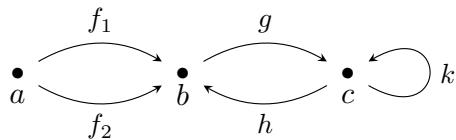
\includegraphics[keepaspectratio]{images/part001_552ae758.jpg}}

represents a quiver whose vertices are a, b, c, and whose arrows are \(f_{1}, f_{2}, g, h, k\) and the source and target maps are given by

\[
\begin{array}{c c c c} o (f _ {1}) = o (f _ {2}) = a & \quad o (g) = b & \quad o (h) = c & \quad o (k) = c \\ t (f _ {1}) = t (f _ {2}) = b & \quad t (g) = c & \quad t (h) = b & \quad t (k) = c. \end{array}
\]

\subsection{Subquivers}

Let C and C′ be quivers. We say that C′ is a subquiver of C if we have \(\operatorname{Som}(\mathrm{C}') \subset \operatorname{Som}(\mathrm{C})\) , \(\operatorname{Fl}(\mathrm{C}') \subset \operatorname{Fl}(\mathrm{C})\) and that the maps \(o_{C'}\) and \(t_{C'}\) coincide with the maps \(o_{C}\) and \(t_{C}\) on \(\operatorname{Fl}(\mathrm{C}')\) . If, moreover, every arrow of C whose source and target belong to \(\operatorname{Som}(\mathrm{C}')\) is an arrow of C', one says that C' is a full subquiver of C.

Let C be a quiver and let \((\mathrm{C}_{i})_{i\in\mathrm{I}}\) be a family of subquivers of C. One calls the intersection of the family \((\mathrm{C}_{i})_{i\in\mathrm{I}}\) and denotes by \(\bigcap_{i\in I}C_{i}\) the subquiver of C whose set of vertices is \(\bigcap_{i\in I}\mathrm{Som}(\mathrm{C}_{i})\) and whose set of arrows is \(\bigcap_{i\in I}\mathrm{Fl}(\mathrm{C}_{i})\) .

\subsection{Morphisms of quivers}

Let C and C' be quivers. A morphism of quivers from C to C' is a pair \((u,v)\) , where \(u\colon\operatorname{Som}(\mathrm{C})\to\operatorname{Som}(\mathrm{C}')\) and \(v\colon\operatorname{Fl}(\mathrm{C})\to\operatorname{Fl}(\mathrm{C}')\) are maps such that \(o_{C'}\circ v=u\circ o_{C}\) and \(t_{C'}\circ v=u\circ t_{C}\) .

Let \(\varphi = (u, v)\) be a morphism of quivers from C to C'. The maps \(u\) and \(v\) are denoted \(\operatorname{Som}(\varphi)\) and \(\operatorname{Fl}(\varphi)\) . If \(a\) is a vertex of C, one will denote, by abuse of notation, \(\varphi(a)\) the image of the vertex \(a\) under \(\varphi\) and we will say that \(\varphi(a)\)

is the image of \(a\) under \(\varphi\) . Similarly, if \(f\) is an arrow of C, we will denote, by abuse of notation, \(\varphi(f)\) the arrow \(v(f)\) of C' and we will say that it is the image of \(f\) under \(\varphi\) .

Let C, \(C'\) , \(C''\) be three quivers, namely \(\varphi = (u, v)\) a morphism from C to \(C'\) and let \(\varphi' = (u', v')\) be a morphism from \(C'\) to \(C''\) . Then \((u' \circ u, v' \circ v)\) is a morphism from C to \(C''\) , denoted \(\varphi' \circ \varphi\) and which is called the composite of \(\varphi'\) and of \(\varphi\) .

We denote \(\mathrm{Id}_{\mathrm{C}}\) the morphism \((\mathrm{Id}_{\mathrm{Som}(\mathrm{C})}, \mathrm{Id}_{\mathrm{Fl}(\mathrm{C})})\) from C into itself.

Let \(\varphi\) be a quiver morphism from C to C'. For \(\varphi\) to be an isomorphism, it is necessary and sufficient that the maps \(\operatorname{Som}(\varphi)\) and \(\operatorname{Fl}(\varphi)\) are bijective (cf. E, IV, p. 6).

Thus, if one calls a quiver structure on sets S and F the data of two maps \(o, t: \mathrm{F} \to \mathrm{S}\) one can take quiver morphisms as morphisms of this structure (E, IV, p. 11).

Let \(\varphi\) be a quiver morphism from C to C'. There exists a unique subquiver of C' whose sets of vertices and arrows are the images of \(\mathrm{Som}(\varphi)\) and \(\mathrm{Fl}(\varphi)\) respectively. It is denoted \(\varphi(\mathrm{C})\) and it is called the image of C under \(\varphi\) . One says that \(\varphi\) is injective if the maps \(\mathrm{Som}(\varphi)\) and \(\mathrm{Fl}(\varphi)\) are injective; in this case, \(\varphi\) induces an isomorphism from C onto its image.

Let \(\varphi\) and \(\psi\) be morphisms of quivers from C to C'. There exists a unique subquiver of C whose vertices and arrows are respectively the vertices and arrows of C having the same image under \(\varphi\) and \(\psi\) . We call it the equalizer of \(\varphi\) and \(\psi\) .

\subsection{Products of quivers}

Let \((\mathrm{C}_{i})_{i\in\mathrm{I}}\) be a family of quivers. Set \(S = \prod_{i\in\mathrm{I}} \mathrm{Som}(\mathrm{C}_{i})\) , \(F = \prod_{i\in\mathrm{I}} \mathrm{Fl}(\mathrm{C}_{i})\) and let o and t be the maps \(\prod_{i\in\mathrm{I}} o_{C_{i}}\) and \(\prod_{i\in\mathrm{I}} t_{C_{i}}\) respectively. The quadruplet \(C = (S, F, o, t)\) is a quiver called the product quiver of the family \((\mathrm{C}_{i})_{i\in\mathrm{I}}\) .

There exists a unique quiver morphism \(pr_{i}: C \to C_{i}\) such that the maps \(\operatorname{Som}(\operatorname{pr}_{i})\) and \(\operatorname{Fl}(\operatorname{pr}_{i})\) are respectively the index-i projections of \(\operatorname{Som}(C)\) onto \(\operatorname{Som}(C_{i})\) and of \(\operatorname{Fl}(C)\) onto \(\operatorname{Fl}(C_{i})\) .

We have the following universal property: Let C' be a quiver; for any family \((\varphi_{i})_{i\in\mathrm{I}}\) where, for every \(i\in I\) , \(\varphi_{i}\colon C'\to C_{i}\) is a quiver morphism, there exists a unique quiver morphism \(\varphi\colon\mathrm{C}^{\prime}\to\mathrm{C}\) such that \(\varphi_{i}=\mathrm{pr}_{i}\circ\varphi\) for all \(i\in\mathrm{I}\) .

\subsection{Paths and loops in a quiver}

DEFINITION 2. --- Let C be a quiver. A path in C is a sequence \(c = (a_{0}, f_{1}, a_{1}, \ldots, a_{n-1}, f_{n}, a_{n})\) , where \(n\) is an integer \(\geqslant 0\) , \(a_{0}, \ldots, a_{n}\) are vertices of C and where, for \(1 \leqslant i \leqslant n\) , \(f_{i}\) is an arrow of C connecting \(a_{i-1}\) to \(a_{i}\) . We say that the path c has length \(n\) .

Let \(c = (a_{0}, f_{1}, a_{1}, \ldots, a_{n-1}, f_{n}, a_{n})\) be a path of length n in C. The vertex \(a_{0}\) is called the origin, or source, of c; the vertex \(a_{n}\) is called the term, or the target, of c; one also says that c joins the vertex \(a_{0}\) to the vertex \(a_{n}\) . The vertex \(a_{i}\) , for \(0 \leqslant i \leqslant n\) , is called the vertex of index i; the arrow \(f_{i}\) , for \(1 \leqslant i \leqslant n\) , is called the i-th arrow, or the arrow of index i. A path of length \(\geqslant 1\) is determined by the sequence of its arrows.

A path whose origin is equal to its endpoint is called a loop. A path of length 0 is a loop, said to be constant.

We say that paths

\[
c = (a _ {0}, f _ {1}, a _ {1}, \ldots , a _ {n - 1}, f _ {n}, a _ {n}) \text{and} c ^ {\prime} = (a _ {0} ^ {\prime}, f _ {1} ^ {\prime}, a _ {1} ^ {\prime}, \ldots , a _ {m - 1} ^ {\prime}, f _ {m} ^ {\prime}, a _ {m} ^ {\prime})
\]

in C are juxtaposable if the endpoint \(a_{n}\) of c is the origin \(a_{0}^{\prime}\) of \(c^{\prime}\) . In this case, the sequence \((a_{0}, f_{1}, a_{1}, \ldots, a_{n-1}, f_{n}, a_{n}, f_{1}^{\prime}, a_{1}^{\prime}, \ldots, f_{m}^{\prime}, a_{m}^{\prime})\) is a path in C, denoted \(c * c^{\prime}\) and called the juxtaposed path of c and \(c^{\prime}\) . It joins the origin of c to the endpoint of \(c^{\prime}\) ; its length is the sum of the lengths of the paths c and \(c^{\prime}\) .

\subsection{Connected components of a quiver}

Let \(C = (S, F, o, t)\) be a quiver. Consider the equivalence relation \(R_{C}\) on S, the finest such that the relation \(\mathrm{R}_{\mathrm{C}}\{o(f), t(f)\}\) is satisfied for every arrow f of C. Two vertices a, b of C are equivalent for this relation if and only if there exists an integer \(n \geqslant 0\) , vertices \(a_{0}, \ldots, a_{n}\) of C and arrows \(f_{1}, \ldots, f_{n}\) of C such that \(a_{0} = a\) , \(a_{n} = b\) and such that, for \(1 \leqslant i \leqslant n\) , the arrow \(f_{i}\) joins either \(a_{i-1}\) to \(a_{i}\) , or \(a_{i}\) to \(a_{i-1}\) .

The equivalence classes of this equivalence relation are called the connected components of C. We denote by \(\pi_0(\mathrm{C})\) the set of connected components of C. Finally, we say that C is connected if it has at most one connected component.

Let \(\varphi\colon\mathrm{C}\to\mathrm{C}^{\prime}\) be a morphism of quivers. The map \(\operatorname{Som}(\varphi)\) defines, by passing to quotients, a map from \(\pi_{0}(\mathrm{C})\) to \(\pi_{0}(\mathrm{C}^{\prime})\) which we denote \(\pi_{0}(\varphi)\) .

\section{GRAPHS}

\subsection{Definition of a graph}

DEFINITION 1. --- A graph \(^{(1)}\) is a quiver (S, F, o, t) equipped with an involution of F, denoted \(f \mapsto \overline{f}\) , without fixed point and such that \(t(\overline{f}) = o(f)\) for all \(f \in F\) .

The quiver (S, F, o, t) is said to be underlying this graph. For every arrow f of this quiver, we have, by definition, \(\overline{\overline{f}} = f\) , \(\overline{f} \neq f\) and \(t(\overline{f}) = o(f)\) . By applying this last relation to the arrow \(\overline{f}\) , one obtains the equality \(o(\overline{f}) = t(f)\) . The arrow \(\overline{f}\) is called the arrow opposite to f.

A pair of opposite arrows of the graph is called an edge of the graph. Each of the two arrows belonging to this pair is called an orientation of this edge. For this reason, the arrows of a graph are also called the oriented edges of the graph.

If G and G' are graphs, a graph morphism from G to G' is a quiver morphism \(\varphi\colon\mathrm{G}\to\mathrm{G}'\) such that \(\overline{\varphi(f)}=\varphi(\overline{f})\) for every arrow \(f\) of G.

Let G and G' be graphs; one says that G' is a subgraph of G if it is a subquiver and if the involution of Fl(G') is the restriction of that of Fl(G).

\subsection{Orientation of a graph}

Let G be a graph. An orientation of G is a subset A of the set of arrows of G such that \(A \cap \overline{A} = \varnothing\) and \(A \cup \overline{A} = \mathrm{Fl}(G)\) .

A graph equipped with an orientation is called an oriented graph.

Let G be an oriented graph and let A be its orientation; an oriented subgraph of G is a subgraph \(G'\) of G equipped with the orientation \(A' = \mathrm{Fl}(G') \cap A\) .

Let (G, A) and (G', A') be oriented graphs. A morphism of oriented graphs from (G, A) to (G', A') is a graph morphism \(\varphi\colon G \to G'\) such that \(\operatorname{Fl}(\varphi)(A) \subset A'\) .

\subsection{Oriented graphs and quivers}

Let G be a graph, \((S,F,o,t)\) the underlying quiver, and A an orientation of G. Then, \((S,A,o\mid A,t\mid A)\) is a quiver, called the quiver associated with the oriented graph \((G,A)\) .

Conversely, let \(C = (S, F, o, t)\) be a quiver. Set \(\widetilde{F} = F \times \{-1, 1\}\) and let \(\widetilde{o}, \widetilde{t}\) be the maps from \(\widetilde{F}\) to S defined by

\[
\begin{array}{l l} \widetilde {o} (f, 1) = o (f) & \qquad \qquad \widetilde {o} (f, - 1) = t (f) \\ \widetilde {t} (f, 1) = t (f) & \qquad \qquad \widetilde {t} (f, - 1) = o (f), \end{array}
\]

for every \(f \in \mathrm{F}\) . Then, \(\widetilde{\mathrm{C}} = (\mathrm{S}, \widetilde{\mathrm{F}}, \widetilde{o}, \widetilde{t})\) , equipped with the involution \((f, \varepsilon) \mapsto (f, -\varepsilon)\) of \(\widetilde{\mathrm{F}}\) is a graph, called the graph associated with the quiver C. The set \(\mathrm{A} = \mathrm{F} \times \{1\}\) is an orientation of this graph. One says that \((\widetilde{\mathrm{C}}, \mathrm{A})\) is the oriented graph associated with the quiver C.

If \(f\) is an arrow of C, one also says that \((f,1)\) is the oriented edge of \(\widetilde{C}\) associated with \(f\) and that the pair \(\{(f,1),(f,-1)\}\) is the edge of \(\widetilde{C}\) associated with \(f\) .

If C' is a subquiver of C, the directed graph \(\widetilde{C}'\) is a directed subgraph of \(\widetilde{C}\) .

There exists a unique quiver morphism \(\varphi\) from C to the quiver underlying \(\widetilde{\mathrm{C}}\) such that \(\varphi(f) = (f,1)\) for every arrow \(f\) of C; it is an isomorphism from C onto the quiver associated with the oriented graph ( \(\widetilde{\mathrm{C}}\) , A).

\subsection{Trees}

When one speaks of paths, or of connected components, of a graph, one means the paths or the connected components of the underlying quiver. Two vertices of a graph belong to the same connected component if and only if there exists a path connecting them.

Let G be a graph. If \(c = (a_{0}, f_{1}, a_{1}, \ldots, f_{n}, a_{n})\) is a path in G, the sequence \(\overline{c} = (a_{n}, \overline{f_{n}}, \ldots, a_{1}, \overline{f_{1}}, a_{0})\) is a path in G, called the opposite path to c. Let c and \(c'\) be juxtaposable paths in G; then, \(\overline{c'}\) and \(\overline{c}\) are juxtaposable, and one has \(\overline{c * c'} = \overline{c'} * \overline{c}\) .

A path c in G is said to be without backtracking if there is no pair of consecutive arrows of c that are opposite. Let \(c = (a_{0}, f_{1}, \ldots, f_{n}, a_{n})\) be a path in G connecting \(a_{0}\) and \(a_{n}\) . If, for an integer i such that \(1 \leqslant i < n\) , the arrows \(f_{i}\) and \(f_{i+1}\) are opposite, the path \((a_{0}, f_{1}, \ldots, a_{i-1}, f_{i+2}, \ldots, f_{n}, a_{n})\) is a path in G connecting \(a_{0}\) to \(a_{n}\) whose length is strictly less than that of the path c. By induction, there therefore exists a path without backtracking in G that connects \(a_{0}\) to \(a_{n}\) .

DEFINITION 2. --- A forest is a graph in which every loop without backtracking is a constant loop. A tree is a connected forest.

PROPOSITION 1. --- Let G be a graph. Every forest of G is contained in a maximal forest of G; in particular, there exists a maximal forest of G.

For a forest of G to be maximal, it is necessary and sufficient that its vertex set be equal to the vertex set of G and that its connected components be those of G.

Let \(A_{0}\) be a forest of G. The set of forests of G, equipped with the order relation “A is a subgraph of B,” is inductive. Consequently, there exists a maximal forest of G of which \(A_{0}\) is a subgraph (E, III, p. 21, cor. 1).

The subgraph of G whose vertex set is \(\operatorname{Som}(G)\) and whose arrow set is empty is a forest of G. Hence there exists a maximal forest of G.

Let A be a maximal forest of G. We prove that A and G have the same vertex set. The subgraph of G whose vertex set is \(\operatorname{Som}(G)\) and whose set of arrows is \(\operatorname{Fl}(A)\) is a forest and A is a subgraph of it. Thus we have \(\operatorname{Som}(A) = \operatorname{Som}(G)\) .

We now prove that A and G have the same connected components. Since every arrow of A is an arrow of G, each connected component of A is contained in a connected component of G. Since A and G have the same vertex set, it suffices to show that two vertices of G lying in the same connected component of G lie in the same connected component of A. If this is not the case, the relation \(R_{A}\) , "being in the same connected component of A," is strictly finer than the relation \(R_{G}\) and there exist two vertices of G that are not in the same connected component of A but are nevertheless joined by an arrow f of G. Let B be the directed subgraph of G whose vertex set is \(\operatorname{Som}(G)\) and whose arrow set is \(\mathrm{Fl(A)} \cup \{f, \overline{f}\}\) . Let us prove that B is a forest of G. Let \(c = (a_{0}, f_{1}, \ldots, f_{n}, a_{n})\) be a nonconstant loop without backtracking in B of minimal length. Since A is a forest, the loop c is not a loop in A. Let i (resp. j) be the smallest (resp. the largest) integer of \(\{0, \ldots, n\}\) such that \(a_{0}\) and \(a_{i}\) (resp. \(a_{j}\) and \(a_{n}\) ) are not in the same connected component of A. This means that the arrows \(f_{i}\) and \(f_{j+1}\) are oriented arrows of B associated with the edge \(\{f, \overline{f}\}\) and that they are opposite. Since the loop c has no back-and-forth, \(f_{i+1} \neq \overline{f_{i}}\) , therefore \(i \neq j\) and the path \((a_{i}, f_{i+1}, a_{i+1}, \ldots, f_{j}, a_{j})\) is a non-constant loop without backtracking in B of length < n, contrary to the hypothesis that c is of minimal length. It follows that B is a forest. This contradicts the hypothesis that A is a maximal forest of G.

Let now A be a forest of G such that \(\mathrm{Som}(\mathrm{A}) = \mathrm{Som}(\mathrm{G})\) and \(\pi_{0}(\mathrm{A}) = \pi_{0}(\mathrm{G})\) . Let us prove that this is a maximal forest of G. It suffices to show that if \(f \notin \mathrm{Fl}(\mathrm{A})\) , the subgraph B of G with vertex set \(\mathrm{Som}(\mathrm{G})\) and arrow set \(\mathrm{Fl}(\mathrm{A}) \cup \{f, \overline{f}\}\) is not a forest. By hypothesis, the points \(o(f)\) and \(t(f)\) lie in the same connected component of A; there therefore exists a path c without backtracking in A joining \(o(f)\) to \(t(f)\) . The path \(c * \overline{f}\) is then a loop without backtracking and non-constant in B, which shows that B is not a forest.

COROLLARY. --- A maximal forest of a connected graph is a maximal tree thereof.

Remark 1. --- In LIE, IV, p. 33, appendix, the notion of a combinatorial graph was defined as a pair (A, S), where S is a set and

A a subset of \(\mathfrak{P}(S)\) consisting of two-element sets; the elements of S are called vertices, those of A edges, and two vertices \(x\) and \(y \in S\) are said to be linked if \(\{x, y\}\) is an edge.

To such a combinatorial graph \(\Gamma = (\mathrm{A},\mathrm{S})\) , one associates a graph G whose vertex set is S and whose arrow set \(\widetilde{\mathrm{A}}\) is the subset of \(\mathrm{S}^2\) formed by the pairs of linked vertices, with the source map and the target map coinciding with the first and second projections of \(\mathrm{S}^2\) in S, and the involution \(f\mapsto \overline{f}\) being given by the restriction to \(\widetilde{\mathrm{A}}\) of the map \((x,y)\mapsto (y,x)\) of \(\mathrm{S}^2\) into itself. The map which to an edge \(\{f,\overline{f}\}\) of G associates the set \(\{o(f),t(f)\}\) is a bijection from the set of edges of G onto that of the edges of the combinatorial graph \(\Gamma\) .

Conversely, every graph such that the source and target of every arrow are distinct, and such that an arrow is determined by its source and target, is of this form.

The reader will verify that the notions of connectedness, tree, or forest for a combinatorial graph coincide with the corresponding notions for the graph associated with it.

\section{GROUPOIDS}

\subsection{Categories}

DEFINITION 1. --- Let C be a quiver. Denote by J the set of pairs \((f,g)\) of arrows of C such that \(t(f)=o(g)\) . A composition law in C is a mapping \(m:J\to\mathrm{Fl}(\mathrm{C})\) such that, for every pair \((f,g)\in\mathrm{J}\) , the origin of the arrow \(m(f,g)\) is that of f and its target that of g.

Let C be a quiver equipped with a composition law \(m\) . Two arrows \(f\) and \(g\) such that \(t(f) = o(g)\) are said to be composable; the arrow \(m(f, g)\) is called their composite, or their product, and is often denoted \(f \cdot g\) , or even \(fg\) .

For every vertex \(a\) of C, the set \(\mathrm{C}_{a,a} = \mathrm{Fl}_{a,a}(\mathrm{C})\) , equipped with the map deduced from \(m\) by passing to subsets, is a magma (A, I, p. 1, def. 1).

A family \((f_{i})_{i\in\mathrm{I}}\) of arrows of C, indexed by a finite nonempty totally ordered set I, is said to be composable if, for every pair \((i,j)\) of consecutive elements of I, the arrows \(f_{i}\) and \(f_{j}\) are composable. One defines the product \(\prod_{i\in\mathrm{I}}f_{i}\) of such a family by induction on the cardinality of I as follows (cf. A, I, p. 3):

\begin{enumerate}
\def\labelenumi{(\roman{enumi})}
\item
  if I has a single element \(\omega\) , \(\prod_{i\in I}f_i = f_\omega\) ;
\item
  if I has at least two elements and if \(\omega\) is the smallest element of I, we set \(\prod_{i\in I}f_i = f_\omega \cdot \prod_{i\in I - \{\omega \}}f_i\) .
\end{enumerate}

The composition law \(m\) is said to be associative if one has \(f \cdot (g \cdot h) = (f \cdot g) \cdot h\) for every composable triple \((f, g, h)\) of arrows of C. When the law \(m\) is associative, the product of a sequence \((f_1, \ldots, f_n)\) of \(n\) composable arrows, where \(n\) is an integer \(\geqslant 1\) , is denoted \(f_1 f_2 \ldots f_n\) .

Let \(a\) be a vertex of C. We say that an arrow \(e \in \mathrm{C}_{a,a}\) is an identity element of \(m\) at \(a\) if one has \(ef = f\) for every arrow \(f\) with source \(a\) and \(ge = g\) for every arrow \(g\) with term \(a\) . There exists at most one identity element of \(m\) at \(a\) : if \(e\) and \(e'\) are two of them, one has \(e' = ee' = e\) . When such an identity element exists, it is often denoted \(e_a\) ; it is then an identity element of the magma \(\mathrm{C}_{a,a}\) (A, I, p. 12).

DEFINITION 2. --- A category is a quiver equipped with an associative composition law for which there exists an identity element at each vertex.

Examples. --- 1) Let C be a quiver. Denote by Ch(C) the set of paths in C and by o: Ch(C) → Som(C), t: Ch(C) → Som(C) the maps which, to a path, associate its origin and its terminus. The quadruple \(\Omega_{\mathrm{C}} = (\mathrm{Som}(\mathrm{C}), \mathrm{Ch}(\mathrm{C}), o, t)\) is a quiver. Equip it with the composition law defined by concatenation of paths. This composition law is associative; for every vertex a of C, the constant loop \(e_a = (a)\) with origin a is an identity element at a. Thus, \(\Omega_{\mathrm{C}}\) is a category. It is said to be the category of paths of the quiver C.

\begin{enumerate}
\def\labelenumi{\arabic{enumi})}
\setcounter{enumi}{1}
\tightlist
\item
  Let \(\Sigma\) be a kind of structure in a theory \(\mathcal{T}\) stronger than set theory and let \(\sigma\{x,y,s,u\}\) be a term of \(\mathcal{T}\) satisfying conditions (MO \(_{\text{I}}\) ), (MO \(_{\text{II}}\) ) and (MO \(_{\text{III}}\) ) of E, IV, p. 11. Let S be a set; suppose that every element of S is a pair \((x,s)\), where \(x\) is a set and \(s\) is a structure of species \(\Sigma\) on \(x\) . Let F be the set of mappings \(f\) such that there exist \((x,s)\) and \((y,t)\) in S such that \(f\) is a \(\sigma\) -morphism from \(x\) , equipped with the structure \(s\) , to \(y\) , equipped with the structure \(t\) ; one then sets \(o(f) = (x,s)\) and \(t(f) = (y,t)\) . Endowed with the composition law given by \(m(f,g)=g\circ f\) , the quiver (S,F,o,t) is a category. In this context, the elements of S are rather called objects.
\end{enumerate}

Let C be a category.

For every vertex \(a\) of C, the set \(\mathrm{C}_{a,a}\) , equipped with the composition law \((f,g)\mapsto fg\) , is a monoid with identity element \(e_a\) .

We say that an arrow \(f\) of C is invertible if there exists an arrow \(g\) of C such that \(o(g) = t(f)\) , \(t(g) = o(f)\) and such that \(fg\) and \(gf\) are identity elements at \(o(f)\) and \(t(f)\) respectively. Such an arrow \(g\) is unique (if \(fg = e_{o(f)}\) and \(g'f = e_{t(f)}\) , we have \(g = e_{t(f)}g = (g'f)g = g'(fg) = g'e_{o(f)} = g'\) ) and is called the inverse of \(f\) ; the inverse of an invertible arrow \(f\) is denoted \(f^{-1}\) .

\subsection{Functors}

DEFINITION 3. --- Let C and C' be categories. A functor from C to C' is called a morphism of quivers \(\varphi\colon\mathrm{C}\to\mathrm{C}'\) such that \(\varphi(fg)=\varphi(f)\varphi(g)\) for every pair \((f,g)\) of composable arrows of C.

Let C and C' be categories and let \(\varphi\colon\mathrm{C}\to\mathrm{C}'\) be a functor. Let \(f\) be an arrow of C, \(a\) its origin and \(b\) its target; then, \(\varphi(f)\) is an arrow of C' with origin \(\varphi(a)\) and target \(\varphi(b)\) .

Let C, C', C'' be categories and let \(\varphi\colon\mathrm{C}\to\mathrm{C}'\) and \(\varphi'\colon\mathrm{C}'\to\mathrm{C}''\) be functors. Then, \(\varphi'\circ\varphi\) is a functor.

Let C be a category. Then the morphism of quivers \(Id_{C}\) is a functor.

Let \(\varphi\colon\mathrm{C}\to\mathrm{C}^{\prime}\) be a functor. In order for \(\varphi\) to be an isomorphism, it is necessary and sufficient that the maps \(\operatorname{Som}(\varphi)\) and \(\operatorname{Fl}(\varphi)\) be bijective.

Thus, if one calls a category structure on sets S and F the data of a quiver structure on these sets and of an associative composition law for which there exists at each vertex an identity element, one can take functors as morphisms of the category structure (E, IV, p. 11).

\subsection{Groupoids}

DEFINITION 4. --- A groupoid is a category in which every arrow is invertible.

Let G be a groupoid and let a be a vertex of G. The monoid \(G_{a,a}\) is a group, which we denote by \(G_{a}\) and which we call the isotropy group of G at a.

Let \(a\) and \(b\) be vertices of G and let \(f \in \mathrm{G}_{a,b}\) be an arrow connecting \(a\) to \(b\) . The map \(g \mapsto fgf^{-1}\) is a group isomorphism from \(\mathrm{G}_b\) to \(\mathrm{G}_a\) , denoted \(\operatorname{Int}(f)\) . If \(f\) and \(f'\) are composable arrows of G, we have \(\operatorname{Int}(ff') = \operatorname{Int}(f) \circ \operatorname{Int}(f')\) . The inverse of the isomorphism \(\operatorname{Int}(f)\) is the isomorphism \(\operatorname{Int}(f^{-1})\) .

A morphism of groupoids \(\varphi\colon G\to G'\) is a morphism of categories. Moreover, \(\varphi\) is a groupoid isomorphism if and only if it is a category isomorphism.

Let \(\varphi\colon\mathrm{G}\to\mathrm{G}^{\prime}\) be a groupoid morphism. For every vertex \(a\) of G, the map \(f\mapsto\varphi(f)\) from \(\mathrm{G}_{a}\) to \((\mathrm{G}^{\prime})_{\varphi(a)}\) is a group homomorphism, denoted \(\varphi_{a}\) . In particular, we have \(\varphi(e_{a})=e_{\varphi(a)}\) .

For every arrow \(f\) of G, \(\varphi(f^{-1})\) is the inverse of \(\varphi(f)\) . If \(f\) is an arrow of G connecting a vertex \(a\) to a vertex \(b\) we thus have, for every element \(g \in \mathrm{G}_b\) , the relation \(\operatorname{Int}(\varphi(f))(\varphi(g)) = \varphi(\operatorname{Int}(f)(g))\) .

\subsection{Orbits of a groupoid}

Let G be a groupoid. The connected components of the underlying quiver of G are called the orbits of G. The set of orbits of G is denoted \(\mathrm{Orb}(\mathrm{G})\) ; if \(\varphi: G \to G'\) is a morphism of groupoids, the map \(\pi_{0}(\varphi)\) deduced from \(\varphi\) by passing to the connected components of the associated graphs is generally denoted \(\mathrm{Orb}(\varphi)\) and is called the map deduced from \(\varphi\) by passing to orbits.

A groupoid with exactly one orbit is said to be transitive. If G is a transitive groupoid, the groups \(G_{a}\) , for \(a \in \text{Som}(G)\) , are isomorphic. We say that the groupoid G is simply transitive if it is transitive and if, moreover, the isotropy groups \(G_{a}\) are all reduced to their identity element.

PROPOSITION 1. --- Let G be a groupoid. The relation "there exists an arrow of G connecting a to b" is an equivalence relation on the set of vertices of G, whose equivalence classes are the orbits of G.

Let \(a\) , \(b\) , \(c\) be vertices of G. We have \(e_a \in \mathrm{G}_{a,a}\) ; if \(f \in \mathrm{G}_{a,b}\) , \(f^{-1} \in \mathrm{G}_{b,a}\) ; if \(f \in \mathrm{G}_{a,b}\) and \(g \in \mathrm{G}_{b,c}\) , we have \(fg \in \mathrm{G}_{a,c}\) . This shows that the indicated relation is reflexive, symmetric, and transitive; it is therefore an equivalence relation. The second assertion then follows from the definition of the connected components of a quiver.

\subsection{Examples of groupoids}

\begin{enumerate}
\def\labelenumi{\arabic{enumi})}
\item
  Let G be a group. Denote by \(\mathcal{G}\) the quiver whose set of vertices is reduced to a single element and whose set of arrows is G. Equipped with the composition law induced by that of G, \(\mathcal{G}\) is a groupoid, called the groupoid associated with the group G.
\item
  Let X be a set. Let G be the quiver \((\mathrm{X}, \mathrm{X} \times \mathrm{X}, \mathrm{pr}_{1}, \mathrm{pr}_{2})\) ; define a composition law on G by setting \((x, x') \cdot (x', x'') = (x, x'')\) , if \(x, x', x''\) are elements of X. This law is associative; for every \(x \in X\) , \((x, x)\) is the neutral element at x; the inverse of the arrow \((x, x')\) is the arrow \((x', x)\) . The groupoid thus defined is called the groupoid of pairs of the set X. If X is nonempty, it is simply transitive.
\item
  Let X and S be sets and let \(p \colon \mathrm{X} \to \mathrm{S}\) be a map. For \(a \in \mathrm{S}\) , write \(\mathrm{X}_a = p^{-1}(a)\) . For \(a\) and \(b\) in S, let \(\mathrm{G}_{a,b}\) be the set \(\mathcal{B}(\mathrm{X}_a; \mathrm{X}_b)\) of bijections from \(\mathrm{X}_a\) to \(\mathrm{X}_b\) and let G be the disjoint union of the sets \(\mathrm{G}_{a,b}\) . Let \(o\) and \(t\) be the maps from G to S such that \(o(f) = a\) and \(t(f) = b\) for every element \(f \in \mathrm{G}_{a,b}\) . The quadruple \((\mathrm{S}, \mathrm{G}, o, t)\) is a quiver. Equip it with the composition law defined by \(m(f, g) = g \circ f\) if \(f \in \mathcal{B}(\mathrm{X}_a; \mathrm{X}_b)\) and \(g \in \mathcal{B}(\mathrm{X}_b; \mathrm{X}_c)\) , where \(a, b, c\) are elements of S. This is a groupoid; it is denoted by \(\mathcal{B}(\mathrm{X}, p)\) and it is called the groupoid of permutations of X relative to \(p\) .
\item
  Let \((\mathrm{G}_{i})_{i\in\mathrm{I}}\) be a family of groupoids. Let G denote the product quiver of the family of underlying quivers; for every \(i\in I\) , let \(pr_{i}\colon G\to G_{i}\) be the canonical quiver morphism. There exists a unique composition law in G for which G is a groupoid and such that, for every \(i \in I\) , \(\mathrm{pr}_i\) is a morphism of groupoids. Let \(f = (f_i)_{i \in I}\) and \(g = (g_i)_{i \in I}\) be arrows of G; they are composable if and only if the arrows \(f_i\) and \(g_i\) are composable, for \(i \in I\) . One then has \(fg = (f_i g_i)_{i \in I}\) .
\end{enumerate}

The quiver G, equipped with this composition law, is called the product groupoid of the family \((\mathrm{G}_{i})_{i\in\mathrm{I}}\) . It satisfies the following universal property: for every groupoid \(G'\) and every family \((\varphi_{i})_{i\in\mathrm{I}}\) , where \(\varphi_{i}\) is a morphism of groupoids from \(G'\) to \(G_{i}\) , there exists a unique morphism of groupoids \(\varphi: G'\to G\) such that \(\varphi_{i}=\operatorname{pr}_{i}\circ\varphi\) for all \(i\in I\) .

\begin{enumerate}
\def\labelenumi{\arabic{enumi})}
\setcounter{enumi}{4}
\tightlist
\item
  Let \(((\mathrm{G}_{i})_{i\in\mathrm{I}},(\varphi_{i,j})_{i\prec j})\) be an inductive system of groupoids, indexed by a right-filtering preordered set \((\mathrm{I},\prec)\) , the \(\varphi_{i,j}\) being morphisms of groupoids. Let G be the quiver whose set of vertices is \(\varinjlim_{i}\operatorname{Som}(\mathbf{G}_{i})\) and whose set of arrows is \(\varinjlim_{i}\operatorname{Fl}(\mathbf{G}_{i})\) , the source and target maps being the maps \(\varinjlim_{i}o_{G_{i}}\) and \(\varinjlim_{i}t_{G_{i}}\) respectively. The composition laws of the \(G_{i}\) induce a composition law on G which makes it a groupoid (cf. A, I, p. 114). The canonical maps \(\operatorname{Som}(\mathbf{G}_{i})\to\operatorname{Som}(\mathbf{G})\) and \(\operatorname{Fl}(\mathbf{G}_{i})\to\operatorname{Fl}(\mathbf{G})\) define a morphism of groupoids \(\varphi_{i}\) from \(G_{i}\) to G. If i, j are elements of I such that \(i\prec j\) , we have \(\varphi_{j}\circ\varphi_{i,j}=\varphi_{i}\) . The groupoid G is called the inductive limit of the family of groupoids \(G_{i}\) and is denoted \(\varinjlim_{i}G_{i}\) . It satisfies the following universal property: for every groupoid H and every family \((\psi_{i})_{i\in\mathrm{I}}\) , where, for \(i\in I\) , \(\psi_{i}:G_{i}\to H\) is a morphism of groupoids, such that \(\psi_{j}\circ\varphi_{i,j}=\psi_{i}\) for every pair \((i,j)\) of elements of I such that \(i\prec j\) , there exists a unique morphism of groupoids \(\psi:G\to H\) such that \(\psi_{i}=\psi\circ\varphi_{i}\) .
\end{enumerate}

For the existence of a groupoid satisfying this universal property when one does not assume that the set I is filtering to the right, cf. II, p. 228, exerc. 3.
